\documentclass[12pt]{article}
%DIF LATEXDIFF DIFFERENCE FILE
%DIF DEL 20150325_QC_Paper.tex   Wed Mar 25 19:25:11 2015
%DIF ADD 20150330_QC_Paper.tex   Mon Mar 30 09:12:49 2015
\usepackage{epsfig, epsf, graphicx, subfigure}
\usepackage{graphicx}
\usepackage{pstricks, pst-node, psfrag}
\usepackage{amssymb,amsmath}
\usepackage{verbatim,enumerate}
\usepackage{rotating, lscape}
\usepackage{multirow}
\usepackage{setspace}

\usepackage{hyperref}
\usepackage[square,sort,comma,numbers]{natbib}
%\usepackage{hyperref}

\usepackage[hang, flushmargin]{footmisc}

\setlength{\oddsidemargin}{-0.125in}
\setlength{\topmargin}{-0.5in} \setlength{\textwidth}{6.5in}
\setlength{\textheight}{9in}

\setlength{\textheight}{9in} \setlength{\textwidth}{6.5in}
\setlength{\topmargin}{-40pt} \setlength{\oddsidemargin}{0pt}
\setlength{\evensidemargin}{0pt}
  
\setlength{\textheight}{9.4in} \setlength{\textwidth}{6.8in}
\setlength{\topmargin}{-71pt} \setlength{\oddsidemargin}{0pt}
\setlength{\evensidemargin}{-6pt} \tolerance=500
%\input psfig.tex
\setlength{\topmargin}{-56pt} \setlength{\oddsidemargin}{-6pt}
%%%%%%%%%%%%%%%%%%%%%%%%%%%%%%%%%%%%%%%%%%
\def\wt{\widetilde}
\def\diag{\hbox{diag}}
\def\wh{\widehat}
\def\AIC{\hbox{AIC}}
\def\BIC{\hbox{BIC}}
\def\sm{\footnotesize}
%- Makes the section title start with Appendix in the appendix environment
\newcommand{\Appendix}
{%\appendix
\def\thesection{Appendix~\Alph{section}}
%\def\thesubsection{\Alph{section}.\arabic{subsection}}
\def\thesubsection{A.\arabic{subsection}}
}
\def\diag{\hbox{diag}}
\def\log{\hbox{log}}
\def\bias{\hbox{bias}}
\def\Siuu{\boldSigma_{i,uu}}
\def\ANNALS{{\it Annals of Statistics}}
\def\BIOK{{\it Biometrika}}
\def\whT{\widehat{\Theta}}
\def\STATMED{{\it Statistics in Medicine}}
\def\STATSCI{{\it Statistical Science}}
\def\JSPI{{\it Journal of Statistical Planning \&amp; Inference}}
\def\JRSSB{{\it Journal of the Royal Statistical Society, Series B}}
\def\BMCS{{\it Biometrics}}
\def\COMMS{{\it Communications in Statistics, Theory \& Methods}}
\def\JQT{{\it Journal of Quality Technology}}
\def\STIM{{\it Statistics in Medicine}}
\def\TECH{{\it Technometrics}}
\def\AJE{{\it American Journal of Epidemiology}}
\def\JASA{{\it Journal of the American Statistical Association}}
\def\CDA{{\it Computational Statistics \& Data Analysis}}
\def\JCGS{{\it Journal of Computational and Graphical Statistics}}
\def\JCB{{\it Journal of Computational Biology}}
\def\BIOINF{{\it Bioinformatics}}
\def\JAMA{{\it Journal of the American Medical Association}}
\def\JNUTR{{\it Journal of Nutrition}}
\def\JCGS{{\it Journal of Computational and Graphical Statistics}}
\def\LETTERS{{\it Letters in Probability and Statistics}}
\def\JABES{{\it Journal of Agricultural and
                      Environmental Statistics}}
\def\JASA{{\it Journal of the American Statistical Association}}
\def\ANNALS{{\it Annals of Statistics}}
\def\JSPI{{\it Journal of Statistical Planning \& Inference}}
\def\TECH{{\it Technometrics}}
\def\BIOK{{\it Bio\-me\-tri\-ka}}
\def\JRSSB{{\it Journal of the Royal Statistical Society, Series B}}
\def\BMCS{{\it Biometrics}}
\def\COMMS{{\it Communications in Statistics, Series A}}
\def\JQT{{\it Journal of Quality Technology}}
\def\SCAN{{\it Scandinavian Journal of Statistics}}
\def\AJE{{\it American Journal of Epidemiology}}
\def\STIM{{\it Statistics in Medicine}}
\def\ANNALS{{\it Annals of Statistics}}
\def\whT{\widehat{\Theta}}
\def\STATMED{{\it Statistics in Medicine}}
\def\STATSCI{{\it Statistical Science}}
\def\JSPI{{\it Journal of Statistical Planning \& Inference}}
\def\JRSSB{{\it Journal of the Royal Statistical Society, Series B}}
\def\BMCS{{\it Biometrics}}
\def\COMMS{{\it Communications in Statistics, Theory \& Methods}}
\def\JQT{{\it Journal of Quality Technology}}
\def\STIM{{\it Statistics in Medicine}}
\def\TECH{{\it Technometrics}}
\def\AJE{{\it American Journal of Epidemiology}}
\def\JASA{{\it Journal of the American Statistical Association}}
\def\CDA{{\it Computational Statistics \& Data Analysis}}
\def\dfrac#1#2{{\displaystyle{#1\over#2}}}
\def\VS{{\vskip 3mm\noindent}}
\def\boxit#1{\vbox{\hrule\hbox{\vrule\kern6pt
          \vbox{\kern6pt#1\kern6pt}\kern6pt\vrule}\hrule}}
\def\refhg{\hangindent=20pt\hangafter=1}
\def\refmark{\par\vskip 2mm\noindent\refhg}
\def\naive{\hbox{naive}}
\def\itemitem{\par\indent \hangindent2\pahttprindent \textindent}
\def\var{\hbox{var}}
\def\cov{\hbox{cov}}
\def\corr{\hbox{corr}}
\def\trace{\hbox{trace}}
\def\refhg{\hangindent=20pt\hangafter=1}
\def\refmark{\par\vskip 2mm\noindent\refhg}
\def\Normal{\hbox{Normal}}
\def\povr{\buildrel p\over\longrightarrow}
\def\ccdot{{\bullet}}
\def\bse{\begin{eqnarray*}}
\def\ese{\end{eqnarray*}}
\def\be{\begin{eqnarray}}
\def\ee{\end{eqnarray}}
\def\bq{\begin{equation}}
\def\eq{\end{equation}}
\def\bse{\begin{eqnarray*}}
\def\ese{\end{eqnarray*}}
\def\pr{\hbox{pr}}
\def\wh{\widehat}
\def\trans{^{\rm T}}
\def\myalpha{{\cal A}}
\def\th{^{th}}
%%%%%%%%%%%%%%%%%%%%%%%%%%%%%%%%%%%%%%%%%%%%%%%%%%%%%%%%%%%%%%%%%%%%%%%%%%%%%
% Marc Definitions
%%%%%%%%%%%%%%%%%%%%%%%%%%%%%%%%%%%%%%%%%%%%%%%%%%%%%%%%%%%%%%%%%%%%%%%%%%%%%
\renewcommand{\baselinestretch}{1.2} % Change this 1.5 or whatever
\newcommand{\qed}{\hfill\hfill\vbox{\hrule\hbox{\vrule\squarebox
   {.667em}\vrule}\hrule}\smallskip}
\newtheorem{Th}{Theorem}
\newtheorem{Proof}{Proof}
\newtheorem{Mth}{Main Theorem}
\newtheorem{Def}{Definition}
\newtheorem{Rem}{Remark}
\newtheorem{Qes}{Question}
\newtheorem{proposition}{Proposition}
\newtheorem{Lem}{Lemma}
\newtheorem{Cor}{Corollary}
\newtheorem{Exa}{Example}
\newtheorem{Eq}{Equation}
%\renewcommand{\baselinestretch}{1.5}
\def\btheta{{\boldsymbol \theta}}
\def\balpha{{\boldsymbol \alpha}}
\def\bmu{{\boldsymbol \mu}}
\def\bpi{{\boldsymbol \pi}}
\def\x{{\bf x}}
\def\a{{\bf a}}
\def\mA{\mathcal{A}}
\def\mB{\mathcal{B}}
\def\mC{\mathcal{C}}
\def\mH{\mathcal{H}}
\def\mR{\mathcal{R}}
\def\mD{\mathcal{D}}

\newtheorem{lemm}{Lemma}[section]
\newtheorem{thm}{Theorem}[section]
\newtheorem{cor}{Corollary}[thm]
\newtheorem{defi}{Definition}
\newtheorem{prop}{Proposition}
\newtheorem{example}{Example}

\def\bX{{\bf X}}
\def\bY{{\bf Y}}
\def\bZ{{\bf Z}}
\def\bU{{\bf U}}
\def\bT{{\bf T}}
\def\bV{{\bf V}}
\def\bx{{\bf x}}
\def\by{{\bf y}}
\def\bz{{\bf z}}
\def\bu{{\bf u}}
\def\bv{{\bf v}}
\def\bs{{\bf s}}
\def\ba{{\bf a}}
\def\bb{{\bf b}}
\def\bmu{{\boldsymbol \mu}}
\def\bbeta{{\boldsymbol \beta}}
\def\balpha{{\boldsymbol \alpha}}
\def\bxi{{\boldsymbol \xi}}
\def\bdelta{{\boldsymbol \delta}}
\def\blambda{{\boldsymbol \lambda}}
\def\btheta{{\boldsymbol \theta}}
\def\beeta{{\boldsymbol \eta}}
\def\bupsilon{{\boldsymbol \upsilon}}
\def\R{\mathbb R}


%\newcommand{\pr}{\mbox{Pr}}
%\newcommand{\var}{\mbox{var}}
%\newcommand{\cov}{\mbox{cov}}
%\newcommand{\logit}{\mbox{logit }}
\newcommand{\cp}{\stackrel{\mathcal{P}}{\rightarrow}}
\newcommand{\cl}{\stackrel{\mathcal{D}}{\rightarrow}}
\newcommand{\mystrut}{\vphantom{\int_0^1}}
\newcommand{\p}{\stackrel{p}{\rightarrow}}
\renewcommand{\d}{\stackrel{d}{\rightarrow}}
\newcommand{\condind}{\perp\hspace{-1em}\perp}
\newcommand{\sumi}{\ensuremath{\sum_{i=1}^{n}}}
\newcommand{\sumj}{\ensuremath{\sum_{j=1}^{n}}}
\newcommand{\eff}{\mbox{\scriptsize eff}}
\def\my{\mathcal Y}




\def\nh{\noindent\hangindent=1.5truecm\hangafter=1}
\def\cl{\centerline}
\def\ms{\medskip}
\def\ni{\noindent}
\def\ve{\vfill\eject}

\def\A{{\rm A}}
\def\ab{\allowbreak}
\def\bigmi{\,\big|\,}
\def\cI{{\cal I}}
\def\cT{{\cal T}}
\def\dt{{\dot t}}
\def\da{{\dot a}}
\def\dar{\downarrow}
\def\ddt{{\ddot t}}
\def\de{\delta}
\def\De{\Delta}
\def\ep{\epsilon}
\def\gz{g_0}
\def\ha{{\hat a}}
\def\half{^{1/2}}
\def\hg{{\hat g}}
\def\hth{{\hat\th}}
\def\hatt{{\hat t}}
\def\hom{{\widehat\om}}
\def\hOm{{\widehat\Om}}
\def\lan{\langle}
\def\ran{\rangle}
\def\lfl{\lfloor}
\def\rfl{\rfloor}
\def\mhf{^{-1/2}}
\def\mi{\,|\,}
\def\mo{^{-1}}
\def\mt{^{-2}}
\def\mth{^{-3}}
\def\mtht{^{-3/2}}
\def\om{\omega}
\def\Om{\Omega}
\def\one{^{(1)}}
\def\oqr{{\textstyle{1\over4}}}
\def\otd{{\textstyle{1\over3}}}
\def\ots{{\textstyle{1\over36}}}
\def\part{\partial}
\def\ra{\to}
\def\rai{\ra\infty}
\def\si{\sigma}
\def\Si{\Sigma}
\def\sumi{\sum_i\,}
\def\sumion{\sum_{i=1}^n\,}
\def\sumionu{\sum_{i=1}^\nu\,}
\def\sumj{\sum_j\,}
\def\sumjon{\sum_{j=1}^n\,}
\def\sumjonu{\sum_{j=1}^\nu\,}
\def\sumjonm{\sum_{j=1}^{n-1}\,}
\def\sz{^0}
\def\T{^{{\rm T}}}
\def\th{\theta}
\def\Th{\Theta}
\def\thf{{\textstyle{1\over2}}}
\def\two{^{(2)}}
\def\var{{\rm var}}
\def\z{_0}
\def\R{\mathbb{R}}
\def\bX{\mathbb{X}}
\def\y{\mathbf{y}}
\def\z{\mathbf{z}}
\def\p{\mathbf{p}}
\def\t{\mathbf{t}}
\def\A{\mbox{A}}
\def\v{\mathbf{v}}
\def\u{\mathbf{u}}
\def\s{\mathbf{s}}
\def\w{\mathbf{w}}
\def\eps{{\ensuremath\boldsymbol{\epsilon}}}
\def\sig{{\ensuremath\boldsymbol{\sigma}}}
\def\thet{{\ensuremath\boldsymbol{\theta}}}
\def\bnu{{\ensuremath\boldsymbol{\nu}}}


\def\hsp{{\hspace{.25cm}}}


\pagenumbering{arabic}
%DIF PREAMBLE EXTENSION ADDED BY LATEXDIFF
%DIF UNDERLINE PREAMBLE %DIF PREAMBLE
\RequirePackage[normalem]{ulem} %DIF PREAMBLE
\RequirePackage{color}\definecolor{RED}{rgb}{1,0,0}\definecolor{BLUE}{rgb}{0,0,1} %DIF PREAMBLE
\providecommand{\DIFaddtex}[1]{{\protect\color{blue}\uwave{#1}}} %DIF PREAMBLE
\providecommand{\DIFdeltex}[1]{{\protect\color{red}\sout{#1}}}                      %DIF PREAMBLE
%DIF SAFE PREAMBLE %DIF PREAMBLE
\providecommand{\DIFaddbegin}{} %DIF PREAMBLE
\providecommand{\DIFaddend}{} %DIF PREAMBLE
\providecommand{\DIFdelbegin}{} %DIF PREAMBLE
\providecommand{\DIFdelend}{} %DIF PREAMBLE
%DIF FLOATSAFE PREAMBLE %DIF PREAMBLE
\providecommand{\DIFaddFL}[1]{\DIFadd{#1}} %DIF PREAMBLE
\providecommand{\DIFdelFL}[1]{\DIFdel{#1}} %DIF PREAMBLE
\providecommand{\DIFaddbeginFL}{} %DIF PREAMBLE
\providecommand{\DIFaddendFL}{} %DIF PREAMBLE
\providecommand{\DIFdelbeginFL}{} %DIF PREAMBLE
\providecommand{\DIFdelendFL}{} %DIF PREAMBLE
%DIF END PREAMBLE EXTENSION ADDED BY LATEXDIFF
%DIF PREAMBLE EXTENSION ADDED BY LATEXDIFF
%DIF HYPERREF PREAMBLE %DIF PREAMBLE
\providecommand{\DIFadd}[1]{\texorpdfstring{\DIFaddtex{#1}}{#1}} %DIF PREAMBLE
\providecommand{\DIFdel}[1]{\texorpdfstring{\DIFdeltex{#1}}{}} %DIF PREAMBLE
%DIF END PREAMBLE EXTENSION ADDED BY LATEXDIFF

\begin{document}
\thispagestyle{empty}
\baselineskip=28pt
\vskip 5mm
\begin{center} {\Large{\bf   Simultaneous Treatment of Random and Systematic Errors in the Historical Radiosonde Temperature Archive}}
\end{center}



\baselineskip=12pt
\vskip 5mm

\begin{center}\large
Joshua M. Browning\footnote{ \baselineskip=10pt
Department of Applied Mathematics and Statistics, Colorado School of Mines, Golden, CO 80401,
USA. 303.384.2462, \\E-mail: \{jbrownin, ahering\}@mines.edu} and Amanda S. Hering$^1$




\end{center}

\baselineskip=17pt
\vskip 5mm
\centerline{\today}
\vskip 5mm

%%%%%%%%%%%%%%%%%%%%%%%%%%%%%%%%%%%%%%%%%%%%%%%%%%%%%%%%%%%%%%%%%%%%%%%%
\begin{center}
{\large{\bf Abstract}}
\end{center}

\baselineskip=14pt

%198 words
\ni  The historical radiosonde temperature archive, and indeed any large and lengthy observational dataset, must be quality controlled before it can be used properly.   Most research on quality control for such data focuses on the identification and removal of either systematic errors or random errors without considering an optimal process for treatment of both.  Additionally, little has been done to evaluate  homogenization methods that identify and correct systematic errors when applied to sub-daily data, and no research exists on using robust estimators in homogenization procedures.  In this paper, we simulate realistic radiosonde temperature data and contaminate it with both systematic and random errors.  We then evaluate (1) the performance of several homogenization algorithms, (2) the influence of removing seasonality, and (3) the sequence in which the random and systematic errors are identified and corrected.  We introduce a robust Standard Normal Homogeneity Test (SNHT) and find in simulations that it performs better than the traditional SNHT, and it is better than several other modern alternatives.  Moreover, we find that systematic errors present in the data lead to poorer performance of random error removal algorithms, but the presence of random errors is not as detrimental to the robust SNHT homogenization algorithm.



\begin{singlespacing}
\par\vfill\noindent
{\bf Some keywords:} Change Point Detection; Homogenization; Outlier Detection; Radiosonde Temperature Data

\par\medskip\noindent
{\bf Short title}:  Simultaneous Random and Systematic Error Detection

\end{singlespacing}
\clearpage\pagebreak\newpage \pagenumbering{arabic}
\begin{doublespacing}


\section{Introduction}


Any large dataset whose observations reach far back in time may require treatment for both systematic and random errors. Datasets such as the International Surface Temperature Initiative (ISTI) global land surface databank \cite{rennie14} with over 32,000 stations, and the Integrated Global Radiosonde Archive (IGRA) housed at the National Climatic Data Center (NCDC) \cite{durre06} are examples of such large datasets. Systematic errors can occur when the station location changes; the area surrounding the station becomes urbanized; or the instrumentation is changed. Random errors can occur due to faulty data transmission; sporadic instrumentation problems; keystroke entries; or errors in data management. To illustrate, Figure~\ref{fig:BasicTS} plots the temperature recorded by radiosondes at the 50 mb pressure level at Station 70219 (Bethel, Alaska, USA); this time series appears to have random and possibly systematic errors.  It is important to treat both sources of errors in  large historical datasets as robustly and automatically as possible. In most published research, methods for handling systematic and random errors are presented separately, and opinions among climate and weather scientists differ in terms of which type of error should be handled first.  We use the term \emph{homogenization algorithms} to refer to the process of identifying and correcting systematic errors while \emph{quality control} (QC) methods are used to identify and remove random errors.   The purpose of this study is to shed light on the order in which systematic and random error methods should be applied to such large datasets when  both sources of error are present. In addition, robust estimators in homogenization algorithms when random errors are present have not yet been considered, so these are proposed and investigated as well.

In this paper, we  focus on the Upper Air Database (UADB) housed at the National Center for Atmospheric Research (NCAR). This archive differs from the IGRA archive in that it contains some different stations, and many of the records are older. Since the radiosonde data are the only direct measured values of the upper atmosphere, it is an important resource for studies in climate change \cite{elliott91, eskridge95} and for use as an input to global reanalysis datasets \cite{kalnay96, kanamitsu02}. Currently over 2,000 station locations exist, and atmospheric variables are collected at standard pressure levels as the radiosonde rises through the atmosphere. In large datasets such as these,  error detection methods must be automated since the archives are so large that visual inspections of every station are not feasible.

Many methods have been developed to homogenize radiosonde data, but most are not tested on simulated data with known contamination errors \cite{eskridge95, haimberger07, haimberger12, lanzante96, lanzante03, venema12}.  However, a study was recently conducted by the European Cooperation in Science and Technology to compare many different homogenization methods \cite{venema12}.  A single large, realistic dataset with known change points was simulated, and then researchers were asked to test their homogenization algorithm on the dataset.  As the researchers did not have knowledge of the true change point locations, this experiment provided a way to compare the performance of  these  methods.  Another approach has been to generate realistic radiosonde temperatures using the Hadley Centre's atmospheric model HadAM3, add random Gaussian noise, and then introduce realistic systematic errors to compare homogenization methods \cite{titchner09, thorne11}, but the computational requirements are so great that only a few  realizations can be simulated.

Most homogenization techniques are designed for monthly or annual time series, but radiosonde observations occur, on average, twice daily.  Some of these techniques rely on optimizing an objective function over all possible points at which a systematic error could occur  \cite{killick12, li14, lu10, scott74}.  Referred to in the statistical literature as \emph{change point detection} methods,   many of these approaches are too computationally expensive for daily data and are not designed to work with nonstationary time series.  For example, a strong seasonal and daily trend is present in radiosonde temperatures, making them ill-suited for application of these methods.  Additionally, some methods may only locate proposed change points and may not correct for the difference in means, which is a necessary homogenization step.  In this paper, we compare the Standard Normal Homogeneity Test (SNHT) \cite{alexandersson86}, the PELT algorithm \cite{killick12}, and binary segmentation \cite{scott74} when applied to data with a seasonal trend and for which a seasonal trend has been removed.  We also propose a robust version of the SNHT.

Automated random error detection methods for radiosonde temperature data have not been investigated as thoroughly \cite{durre06,durre08,lanzante96}.  Models such as \cite{ignaccolo14} for  the entire vertical column using pairs of locations could be adapted for random error detection, but  recently  several random error detection methods, corresponding \DIFaddbegin \DIFadd{to }\DIFaddend the climatological check step of \cite{durre08}, for a given location and pressure level are proposed and evaluated with simulated datasets \cite{bell14}. The authors find that the optimal error detection algorithm requires two steps: first scanning for observations that are too many standard deviations from the global mean and secondly scanning for observations that are too many standard deviations from their local mean.  Robust estimators of mean and standard deviation are used in both cases to mitigate the influence of errors, and a robust, asymmetric estimate of standard deviation is introduced to account for skewness in temperature distributions.

However, to our knowledge, no research has been done to date describing which type of error should be handled first when a dataset contains both types of errors.  We do a simulation study in which data is contaminated with both known random errors and with known change points so that we can  evaluate  (1) the performance of our robust SNHT compared to other modern alternatives; (2) the effect of strong seasonality on homogenization methods; and (3) the sequence in which different quality control algorithms are applied.  We henceforth refer to the choice of performing random error detection or systematic error detection first  as ``the sequence of the quality control method'' or simply ``the sequence.''  In Section 2, we discuss the details of our data simulation and contamination.  Section 3 evaluates the performance of the homogenization algorithms we use, and Section 4 gives the results from the sequencing study.  In Section 5, we present a case study of this method applied to a real dataset, and some conclusions are offered in Section 6.  \textbf{[Note--for IJoC submission, remove the references to section numbers in this paragraph.]}

\section{Simulation Method}
Observational data cannot be used to evaluate the performance of  homogenization and QC methods directly since we cannot know exactly where true change points and random errors occur.  Therefore, a rigorous simulation study is developed in order to accurately compare methods and their sequence.  Evaluation of methodology via simulation is commonplace in the statistics literature, and our approach bases the simulation on actual data.  In order for this simulation study to validate methods for radiosonde data, it is crucial that we simulate data that is similar in structure to true radiosonde data.

\subsection{Modeling Radiosonde Data}
\label{ssec:model}

In order to capture seasonal and hourly trends, we fit a Generalized Additive Model (GAM) to  radiosonde temperature data.  GAMs are flexible, non-parametric models that allow the response variable to be a linear combination of smoothed functions of the input variables \cite{hastie90}.  In our case, we model temperature (for a fixed location and pressure level) as a function of hour of day, day of year, and year.  We model the annual trend with a linear term to capture long term increases or decreases in the series.  Thus, the model we fit is
\begin{equation} \label{eq:GAM}
	t_i = \beta_0 + s_1(h_i) + s_2(d_i) + \beta_1 y_i + \epsilon_i,
\end{equation}
\ni where $t_i$ is the temperature at a given station and pressure level; $h_i$, $d_i$, and $y_i$ are the hour, day, and year of the $i$-th observation, respectively; $\beta_0$ is the intercept; $\beta_1$ is the coefficient for the long term trend; and $s_1(\cdot)$ and $s_2(\cdot)$ are cubic regression splines.

Typically the error term, $\epsilon_i$, in Equation~(\ref{eq:GAM}) would be modeled as normal with some unknown variance, but the distribution of the error terms could be skewed or have heavier tails than a normal distribution as shown by \cite{bell14} for radiosonde temperatures.  Thus, we use a skew-$t$ distribution for the errors of this model, which has 4 parameters, $\xi, \sigma, \alpha$, and $\nu$, which are useful in controlling the first four moments of the distribution \cite{azzalini03}.  This distribution is very flexible and can handle skewed and heavy-tailed data.

Additionally, we expect there to be temporal correlation in the error terms.  However, since we have already included hourly and seasonal terms in the model,  most of this autocorrelation is already explained, so an AR(1) time series model is sufficient to account for the remaining structure in the residuals.  This model assumes that each error term has some fixed correlation with the error one time step in the past, and thus can be estimated by simply computing the correlation between $t_i$ and $t_{i+1}$ when the observations are equally spaced.

However, for radiosonde data, observations are not guaranteed to be equally spaced in time.  Launches are scheduled globally at 0 and 12 UTC; however, many deviations from this pattern are observed, especially in the historic record.  Most observations are within an hour or two of the scheduled launches, but in some instances, no launches occur on a given day, and on others, more than two radiosondes are launched.   Thus, to estimate the lag-$h$  autocorrelation, ${\phi}(h)$, in hours, we must use only those observations that are $h$ time steps apart:
\begin{equation} \label{eq:ACF}
	\widehat{\phi}(h)=\frac{1}{\lvert \mathcal{P}_h\rvert} \sum_{(\hat{\epsilon}_i,\hat{\epsilon}_j) \in \mathcal{P}_h} \frac{(\hat{\epsilon}_i-\bar{\epsilon})(\hat{\epsilon}_j-\bar{\epsilon})}{s^2_{\hat\epsilon}},
\end{equation}
\ni where $\mathcal{P}_h$ is the set of all pairs of residuals that are $h$ hours apart (or within some window); $|\mathcal{P}_h|$ is the number of pairs of residuals in the set $\mathcal{P}_h$;  $\hat{\epsilon}_i$ is the observed residual from Equation~(\ref{eq:GAM}); $\bar\epsilon$ is the average of the residuals; and $s^2_{\hat\epsilon}$ is the standard deviation of the residuals.  For an AR(1) model, we need only estimate $\phi(\cdot)$ at $h=12$ hours, and we use a window of 5\% of 12 hours, or 0.6 hours.

\subsection{Data Simulation}
\label{ssec:sim}

The data simulation procedure has seven steps:
\begin{enumerate}
	\item Fit Equation~(\ref{eq:GAM}) to observed radiosonde temperature data at a given location and pressure level.  Then, fit a skew-$t$ distribution to the error terms, and model the autocorrelation with Equation~(\ref{eq:ACF}).
	\item We choose a fixed time period and assume that two observations occur for each day within that time period: one in the morning and one in the evening.  The time of each morning (evening) observation is simulated by sampling a time from the morning (evening) subset of the observed data.  This process is done to ensure that variability in the simulated hour of observation is comparable with that of the observed data.
	\item We use the GAM model fit in step 1 to determine the expected value of temperature at the simulated time, denoted $\hat t_i$.
	\item To simulate the noise in the observations, we randomly draw values $\delta_i$ from a skew-t distribution with parameters as fit in step 1.
	\item We wish to introduce autocorrelation in these $\delta_i$.  Thus, we simulate an AR(1) model via
	\begin{equation*}
	\epsilon_i = \widehat{\phi}(12)^{\Delta_{i-1}/12} \epsilon_{i-1} + \delta_i,
	\end{equation*}
	where $\epsilon_i$ is the simulated noise in the model at time $i$, and $\Delta_{i-1}$ is the time difference, in hours, between the $(i-1)$th and $i$th observation.  Note that the $i$th term in this series will depend on all of the previous $i-1$ values.  To ensure the correct correlation structure, we simulate 1,000 more values than needed and discard the first 1,000.
	\item Then, the simulated $\epsilon_i$ is added to $\hat{t}_i$ to construct a simulated series that is similar to real radiosonde temperatures.

	\item Lastly, we contaminate this data with systematic and random errors.  (a) Random errors are generated by sampling 1, 2, 5 or 10\% of the observations and adding or subtracting a random error following a distribution of $N(10\sigma,1\sigma^2)$, where $\sigma$ is the standard deviation of the simulated series, estimated by the variance of the observed errors in Equation (\ref{eq:GAM}).  (b) Systematic errors are generated by sampling 1, 2, or 3 observations uniformly per simulated decade and then drawing a break size from a $N(0,0.04 \sigma^2)$.  The break size is then added to all observations after the change point.  Both the contaminated and uncontaminated datasets are stored for comparison.  Figure~\ref{fig:simExample} shows an example of one of the radiosonde temperature datasets that we use as a basis for simulation as well as two different realizations of simulated and contaminated datasets.
\end{enumerate}

We vary several additional factors within our data simulation to understand the effect that each factor has on homogenization algorithms and the sequence in which the algorithms are applied.

\textbf{Climate Zones:} Radiosonde temperature data from different climate zones can be dramatically different, and so we analyze data from many different climate zones.  In \cite{bell14}, ten representative stations are chosen and analyzed from ten different climate types, and we simulate data based on models fit to these ten stations.

\textbf{Pressure Level:} Radiosonde temperature data can also vary  over pressure level, and so we analyze the pressure levels chosen in \cite{bell14}: 100 mb, 300 mb, and 850 mb.

\textbf{Sample Size:}  For the sequencing study, sample sizes of twice-daily data are simulated for 20, 40, and 80 years.  The study comparing homogenization algorithms, however, is much more computationally expensive, so we use sample sizes of 10, 20, and 40 years.

\section{Homogenization Algorithms}

Radiosonde observations are collected over long periods of time, as long as 100 years for some stations, and therefore systematic changes in the mean temperature are not uncommon.  These errors can happen for one of many reasons such as changes in instrumentation, relocation of a station, or post-processing of data.  Methods which detect and/or correct these errors are referred to as homogenization algorithms, and many such techniques have been developed by the meteorological community \cite{alexandersson86, domonkos13, gruber08, haimberger07, lanzante03, li14, lu10, venema12}.  Many of the homogenization algorithms make use of metadata, which document changes in the data collection process and/or compare data from neighboring stations.  We do not evaluate such algorithms since we simulate data from one station and pressure level at a time.  In \cite{haimberger07}, SNHT is applied by combining both metadata and the ERA-40, but we use a simplified version that operates purely on the observed data.

In this section, we compare the abilities of four different homogenization algorithms to detect systematic errors when random errors are also present in the data.  We summarize the methods we investigate, namely Binary Segmentation (BinSeg) \cite{scott74}, Pruned Exact Linear Time (PELT) \cite{killick12}, SNHT, and a new robust SNHT.  In addition, we study the performance of these algorithms when the seasonal trend is present versus having been modeled and removed.  We simulate data as described in Section 2 and then introduce change points and random errors, and we evaluate the ability of the algorithms to detect the known change points. 

\subsection{Methodology}
\label{ssec:methodology}

Two algorithms, BinSeg and PELT, detect the number and location of change points by optimizing a cost function of the form
\begin{equation}
	\sum_{i=1}^{m+1} [\mathcal{C}(y_{(\tau_{i-1}+1):\tau_i})] + \beta f(m),
	\label{eq:cost}
\end{equation}
where $\tau_i$ is the $i$th change point; $m$ is the number of change points; $\mathcal{C}$ is a cost function; $y_{(\tau_{i-1}+1):\tau_i}$ is the observed data between the $(i-1)$ and $i$th change point; and $\beta f(m)$ is a penalty term on the number of change points to prevent overfitting \cite{killick12}.  Note that, for notational convenience, $\tau_{m+1}$ is defined to be the last observation.  Often, $\mathcal{C}$ is chosen to be twice the negative log likelihood, and $f(\cdot)$ is linear.

Optimization of Equation (\ref{eq:cost}) can be done in several ways.  BinSeg uses a divide-and-conquer algorithm: each observation is considered a candidate change point, and the one which leads to the largest reduction in the cost function is chosen as a change point.  This change point then segments the data into two groups, and the same procedure is repeated on each segment.  If no observations lead to a reduction in the cost function, then the procedure is terminated.  BinSeg is known to be computationally efficient but is not guaranteed to reach the global minimum of the cost function.

PELT is another algorithm for optimizing Equation (\ref{eq:cost}), but it computes the exact minimum.  It proceeds recursively as follows: first, the optimal number and location of change points is determined for the first two observations  only.  The optimal number and location of change points for the first three observations is then determined using this information, and more generally the optimal number and location of change points for the first $k+1$ observations is determined by considering the optimal configurations for the first $2, 3, \ldots, k$ observations.  PELT is computationally efficient.  For our analysis, we used the BinSeg and PELT algorithms implemented in the \texttt{changepoint} package in R \cite{killick14}.

The SNHT test works as follows.  For each observation, two means are computed: one for the $N$ days prior to observation $i$, $\bar{X}_{L,i}$, and one for the $N$ days following, $\bar{X}_{R,i}$.  Then, the test statistic
\begin{equation}
	T_i = \frac{N}{s_i^2}\left( (\bar{X}_{L,i}-\bar{X}_i)^2 + (\bar{X}_{R,i}-\bar{X}_i)^2\right),
	\label{eq:Hom}
\end{equation}

\ni is computed where $\bar{X}_i$ is the mean of $\bar{X}_{L,i}$ and $\bar{X}_{R,i}$, and $s_i$ is the estimated standard deviation over the $N$ days prior and $N$ days following observation $i$.  If there are not $N$ observations both before and after the current observation, no test is performed.  If the largest $T_i$ exceeds some threshold at time $i=i^*$, we conclude that a change point occurred at time $i^*$, and we adjust all observations after time $i^*$ by $\bar{X}_{L,i^*}-\bar{X}_{R,i^*}$.  Homogenization now proceeds iteratively.  $T_i$ is recomputed for all $i$ that are sufficiently far away from the current change points, $i\in\{1,\ldots,n\} \setminus \{i^*-k, \ldots, i^*+k\}$, and the test is performed again until no $T_i$ exceed the threshold, and we use $k=N$.  Note that in practice, it is generally preferable to homogenize to the most recent data, as that data is considered to be more reliable, and some follow this convention \cite{domonkos13}. %Section 2.3
We note that the test statistic in \cite{haimberger07} differs from Equation~(\ref{eq:Hom}) in that a denominator of $s_i$ is used in place of $s_i^2$; however, we believe this to be a typographical error, as the statistic in \cite{haimberger07} is derived from \cite{alexandersson86}.  In \cite{alexandersson86}, $\bar{X}_{L,i}, \bar{X}_{R,i}$ and $\bar{X}_{i}$ are first standardized, and  this is equivalent to our formulation.

%The test statistic in \cite{haimberger07} differs from the one here in that a denominator of $s_i$ is used in place of $s_i^2$.  However, we believe that to be a typographical error, as the statistic in \cite{haimberger07} is derived from \cite{alexandersson86}.  In \cite{alexandersson86}, $\bar{X}_{L,i}, \bar{X}_{R,i}$ and $\bar{X}_{i}$ are first standardized, and thus this is equivalent to our formulation.  However, for comparison purposes, we homogenize the simulated datasets with both statistics.  For the statistic with $s_i$ in the denominator, a threshold of 100 is recommended, and we find that value to work well in our simulations.

The threshold for determining when a change point has occurred is based on the sampling distribution of Equation~(\ref{eq:Hom}).  We first note that the SNHT algorithm generally makes the assumptions that the observations are independent and \DIFdelbegin \DIFdel{approximately }\DIFdelend normal with some fixed mean\DIFdelbegin \DIFdel{, which imply that the statistic follows a chi-squared distribution with two degrees of freedom, i.e.  , $T_i\sim \chi^2_2$.  }\textbf{%DIFDELCMD < [%%%
\DIFdel{Josh--triple-check based on the Alexandersson paper.}%DIFDELCMD < ]%%%
}  %DIFAUXCMD
\DIFdelend \DIFaddbegin \DIFadd{.  Under these assumptions, 
}\begin{equation*}\DIFadd{
	\frac{N}{2 \sigma^2}\left( (\bar{X}_{L,i}-\bar{X}_{R,i})^2\right) \sim \chi^2_1,
}\end{equation*}
\DIFadd{\ni where $\sigma^2$ is the variance of the $X_i$.  If we replace $\sigma^2$ with $s_i^2$ we get our test statistic, and so $T_i$ is approximately $\chi^2_1$.  }\DIFaddend However, these assumptions do not all hold for radiosonde temperature data, as temperatures follow seasonal trends, which induce a strong dependence among the observations.  Thus, homogenization will likely be improved if the seasonal components of the data are removed.  We use a model-based approach to removing the seasonality; however, we  chose a model simple enough so that it does not inadvertently remove change points, as a pure linear trend would.  Thus, we use a GAM model of the form
\begin{equation}\label{eq:season}
	t_i = \beta_0 + s_1(d_i) + \epsilon_i
\end{equation}
where $t_i$ is the temperature at a given station and pressure level, $d_i$ is the day of the year of the $i$-th observation, $\beta_0$ is the intercept, $\epsilon_i$ is the error of the model, and $s_1$ is a cubic regression spline.   We then subtract this fit from the data, giving errors about an estimated seasonal mean.  These errors will no longer exhibit a seasonal trend, and thus the assumptions of independent and mean-zero observations are much more reasonable.  This simple model was chosen because it will leave the numerator of the SNHT statistic unchanged, as the same adjustment will be applied to the observations before $t_i$ as the observations after.  However, a more reasonable estimate for $s_i$ can now be obtained, and the distribution of the  SNHT statistic is more closely approximated by a chi-squared with \DIFdelbegin %DIFDELCMD < {%%%
\DIFdel{two}%DIFDELCMD < } %%%
\DIFdel{degrees }\DIFdelend \DIFaddbegin \DIFadd{one degree }\DIFaddend of freedom.  We use the 99\% quantile of this distribution as our threshold.  Moreover, the SNHT statistic is applied many times to the same time series, so we use the Benjamini-Hochberg adjustment for multiple testing of dependent tests to ensure that the family-wise Type I error rate remains below the 1\% threshold \cite{benjamini01}.

We now propose a robust version of the SNHT wherein we replace the means and standard deviation in Equation~(\ref{eq:Hom}) with the Huber M-estimator of the mean and standard deviation \cite{huber11}.  These robust estimators of center and spread are computed as follows:
\begin{enumerate}
	\item First, the estimates of the mean, $\hat{\mu}$, and standard deviation, $\hat{\sigma}$, are initialized to
	\begin{align*}
		\hat{\mu} &= \mbox{median}(\mathbf{x})\\
		\hat{\sigma} &= \mbox{MAD}(\mathbf{x}),
	\end{align*}
	where $\mathbf{x}$ is a vector of the data, and $MAD$ is the median absolute deviation, defined as
	\begin{equation*}
		MAD = \mbox{median}( \lvert x_i - \mbox{median}(\mathbf{x}) \rvert ).
	\end{equation*}
	\item Then, Winsorized values, $y_i$, are computed.  These are defined as
	\begin{equation*}
		y_i = \left\{ \begin{array}{ll}
			\hat{\mu}-k \hat{\sigma} & : x_i \leq \hat{\mu}-k \hat{\sigma}\\
			x_i & : \hat{\mu}-k \hat{\sigma} < x_i \leq \hat{\mu}+k \hat{\sigma}\\
			\hat{\mu}+k \hat{\sigma} & : x_i > \hat{\mu}+k \hat{\sigma},\\
		\end{array} \right.
	\end{equation*}
	and $k$ is commonly taken to be 1.5, which is what we use.
	\item Updated estimates of $\hat{\mu}$ and $\hat{\sigma}$ are computed as the mean of $\mathbf{y}$ and the standard deviation of $\mathbf{y}$, respectively.
	\item Steps 2 and 3 are repeated until $\hat{\mu}$ changes by less than $10^{-6} \hat{\sigma}$.
\end{enumerate}

\ni This definition forces unusually large observations to have little to no influence on the estimators of the mean and standard deviation, and they are robust against random errors, which may be present during homogenization.  BinSeg and PELT are not robust against random errors when $\mathcal{C}$ is chosen to be twice the negative Gaussian log likelihood.  An \texttt{R} package implementing the robust SNHT is available on CRAN at \url{http://cran.r-project.org/web/packages/snht/index.html}.

Evaluation of homogenization algorithms can be done by computing the number of simulated change points in the data that were accurately detected.  However, it is unlikely that a homogenization algorithm will detect the exact time of the change point, and thus hit rate is not a very useful metric.  Instead, we use efficiency as defined in \cite{domonkos13}.  Let $\mathbf{x}$, $\mathbf{c}$, and $\mathbf{h}$ be the original, contaminated, and contaminated and homogenized time series, respectively and let the $i$-th observation be denoted by $x_i, c_i$, and $h_i$ respectively.  The Root Mean Square Error (RMSE) of $\mathbf{h}$ is then defined as follows:
\begin{equation*}
	\mbox{RMSE}(\mathbf{h}) = \sqrt{\frac{1}{n} \sum_{i=1}^n (h_i-x_i)^2}.
\end{equation*}
Then, the efficiency of the homogenized series, where 1 means perfect skill, 0 means no improvement, and negative values indicate degradation is
\begin{equation*}
	\mbox{Eff}(\mathbf{h}) = \frac{\mbox{RMSE}(\mathbf{c})-\mbox{RMSE}(\mathbf{h})}{\mbox{RMSE}(\mathbf{c})}.
\end{equation*}
The homogenization algorithm is not designed to locate or correct random errors.  Furthermore, random errors in the data introduce variability in the estimate of efficiency, so we remove the random errors in $\mathbf{c}$ and $\mathbf{h}$ before computing the RMSE scores.  

We compare the efficiency of all four different homogenization algorithms on simulated datasets.  The simulated datasets are  either 10, 20, or 40 years long, and change point locations are simulated uniformly at random across the entire time series excluding the first and last year.  We simulate either one, two, or three change points per decade.  All of the homogenization algorithms considered have tuning parameters: for PELT and BinSeg we must choose penalty functions and the $\beta$ constant, and for SNHT and its robust variant we must specify the period $N$.  Thus, in our simulations we vary the following tuning parameters to observe their effect on the overall performance:

\begin{itemize}
	\item PELT: We consider penalties of $\beta=n/2$, $n$, $2n$, $4n$, and  $8n$.
	\item BinSeg: We use no penalty term and instead restrict the maximum number of change points that can occur, varying from 1 to 10.
	\item SNHT: This algorithm computes means of seasonal data, so periods which are multiples of a year should be considered.  Thus, we use one and two year averaging windows with $N=365$ or $N=730$.
	\item Robust SNHT: We  use $N=365$ and $N= 730$.
\end{itemize}

In summary, the simulation process is as follows:

\begin{enumerate}
	\item Simulate and contaminate data as described in Section~\ref{ssec:sim}.
	\item Apply each homogenization algorithm to the contaminated dataset.  Counting all of the homogenization algorithms along with each one's unique tuning parameters, we apply   a total of 19 different homogenization algorithms. Since each is applied to both the original and detrended data, we have 38 different methods to compare.
	\item Store the efficiency of each method.
	\item Steps 1-3 are repeated 500 times for each combination of climate zone, pressure level, and sample size.
\end{enumerate}

\subsection{Results}

\label{sec:HomResults}

Figure~\ref{fig:homEfficiency} depicts a boxplot of the efficiencies measured for each of the different algorithms across all 90,000 simulations, i.e.~ for 500 simulations at each of 3 pressure levels, 10 stations, 3 sample sizes, and 2 seasonal removal (detrended or not) configurations.  The robust version of the SNHT appears to achieve the best efficiency among all homogenization algorithms considered.  The BinSeg algorithms perform best when we force the algorithm to choose a small number of change points.  However, in practice, we will not know the true number of change points, and the BinSeg algorithm is very sensitive to this choice.  The PELT algorithm appears to perform best with a penalty of $n/2$, but its performance is  worse than the alternative algorithms.  Removing the seasonal trend generally improves the efficiency of the algorithms; however, the improvement is greatest for the algorithms with lower efficiency.

To further understand the performance of these algorithms and to understand their sensitivity to different simulation parameters, we fit a logistic regression model to the simulation results.  The response variable is 1 if efficiency is positive and 0 otherwise, and the independent variables we use are the sample size $n$, the outlier contamination rate, the station, the pressure level, the homogenization algorithm, and if a seasonal adjustment was applied.  We fit 4 different logistic regression models: first one with main effects and then models with $k$-way interactions, where $k=2,3,4$.  Table~\ref{tab:homOrdDev} reports the deviance, a measure of logistic regression model fit, for each model.  As the deviance does not decrease substantially after $k$ increases beyond 2, we use the model with only 2-way interaction terms.

Table~\ref{tab:homOrd} displays the average fitted efficiency as a function of $n$, outlier contamination, and homogenization method.  Only the most promising methods from  Figure~\ref{fig:homEfficiency} are displayed here, and the first set of columns are the estimated efficiencies when the seasonality is not removed.  The second set of columns shows the increase in fitted efficiency when the seasonality is first removed with Equation~(\ref{eq:season}).   The first number indicates the fitted efficiency, averaged across all station and pressure level combinations, and the number in parentheses indicates the proportion of station and pressure level combinations where this model attains the highest fitted efficiency.  The robust SNHT with seasonal trend removed is the superior model in almost all scenarios.  However, the traditional SNHT is occasionally better when the outlier contamination rate is small (0\% or 1\%).  The robust SNHT with a 730 day period performs slightly better on the 40 year datasets but not enough to warrant its use.  However, this suggests that it may be optimal if many years of data are available. Almost all of the methods are improved by detrending first, but the SNHT and robust SNHT are not nearly as affected by detrending.  The BinSeg method  is improved by over 20\% for small sample sizes with the gain decreasing as the outlier contamination increases.  Based on these results, we use the robust SNHT for the remainder of this paper with $N=365$ and seasonal trend removed.

Plots of the fitted probability that efficiency is positive are given in Figure~\ref{fig:homFitEff}.  Each individual line represents a different simulation configuration (number of years simulated and outlier contamination rate).  As seen previously, this plot shows that the SNHT and robust SNHT attain the highest fitted probabilities in all cases.  Also, the efficiency generally improves as the sample size increases.

\section{Sequencing Study}

Many radiosonde temperature datasets have observations collected over long periods of time.  Thus, it is possible and likely that both systematic and random errors exist in the data.  It is not clear if random errors should be removed from the data prior to systematic errors, or vice versa.  Thus, this simulation study investigates the performance of different sequences of these quality control methods.

\subsection{Random Error Detection}
\label{sec:ranErr}
We follow the random error identification process developed and tested in \cite{bell14}.  Given that errors are present in the data, traditional methods of computing the mean and standard deviation are known to perform poorly.  Thus, the authors use the two-sided Huber estimator, which produces a robust measure of the location and robust measures of scale for both the left and right sides of the distribution \cite{huber11}.  The two-sided Huber estimator differs from the estimator described in Section~\ref{ssec:methodology} only in that it produces two estimates of scale, $\sigma_R$ and $\sigma_L$.  The estimate for $\sigma_R$ ($\sigma_L$) is computed using only the data to the right (left) of $\hat{\mu}$.

Anderson et al.~\cite{bell14} investigate several different strategies for selecting subsets of observations with which to estimate the Huber mean and standard deviations.  The \emph{Global} set uses all of the observations to estimate the parameters, and the \emph{Hourly Combined} set takes all observations within  a 45 day and 12 hour window of each observation across all years and computes parameter estimates for each one.  Their final algorithm first removes observations whose $z$-scores based on the Global parameter estimates are greater than 6, and then removes observations whose $z$-scores  based on the Hourly Combined parameter estimates exceed 5.  

%detection methods that estimate the Huber mean and standard deviations on different subsets of the data.  These subsets are defined by moving daily windows and hourly groupings, as well as considering a global approach which uses all observations.  We examine each method and agree with the authors that the best method was the  ``Hourly Combined.''  This approach searches for errors using the entire dataset first and then computes the estimators on subsets defined by hourly groupings and daily windows.

\subsection{Sequencing Simulation}

We apply four different sequencings of homogenization and random error identification to the data: homogenization followed by random error detection; random error detection followed by homogenization; homogenization followed by random error detection followed by homogenization; and random error detection followed by homogenization followed by random error detection.  We refer to these approaches as ``Sys-Ran,'' ``Ran-Sys,'' ``Sys-Ran-Sys,'' and ``Ran-Sys-Ran,'' respectively.

We hypothesize that some random errors will not be detected if the data is not homogenized and that the homogenization procedure will not perform as well if random errors are not first removed.  For these reasons, we included the two additional methods ``Sys-Ran-Sys'' and ``Ran-Sys-Ran''.  In both of these approaches, a homogenization procedure is performed after random error detection.  Likewise, a random error detection will be performed after a homogenization algorithm as well.

In summary, the simulation process is as follows:

\begin{enumerate}
	\item Simulate and contaminate data as described in Section~\ref{ssec:sim}.
	\item Apply each sequencing of the quality control process.
	\item Store the true and false positive rate for random error detection as well as the efficiency of the homogenization algorithm.  The true positive rate, TPR, is defined as the percent of identified errors that are random errors, and the false positive rate, FPR, is defined as the percent of identified errors that are not random errors.
	\item Steps 1-3 are repeated 1,000 times for each climate zone,  pressure level, and sample size.
\end{enumerate}

\subsection{Sequencing Results}

The percent of error contamination as well as the number of simulated change points in the data can strongly influence TPR and FPR.  Thus, we again fit logistic regression models to the simulation results, where we model each of TPR, FPR, and the probability that efficiency is positive as the response variables.  The dependent variables are sample size, outlier contamination rate, station, pressure level, and sequencing.

We begin by fitting five logistic models for each of the three responses, first with only main effects and then models with all $k$-way interaction terms, where $k=2,3,4,5$.  The deviances are given in Table~\ref{tab:devSeq}.  We again find that the deviance does not decrease much when 3-way interaction terms are included in the model, and thus we use models with 2-way interaction terms for all three responses.

For the TPR model, we find that there is no significant difference between the sequencings ``Ran-Sys-Ran,'' ``Sys-Ran,'' and ``Sys-Ran-Sys.''  Table~\ref{tab:fitTPR} shows the fitted TPR averaged across all stations and pressure levels, and the number in parentheses shows the percent of instances when that model attains the highest fitted TPR.  Additionally, these effects are plotted in Figure~\ref{fig:fitTPR}.  The table shows that the ``Ran-Sys'' sequencing performs best when the outlier contamination rate is small and when the sample size is relatively small.  The other sequences perform  similarly and do much better than the ``Ran-Sys" sequence when the sample size is medium to large and as the outlier contamination rate increases.  

For the FPR model, we did not find a substantial difference among the four sequencings.  Table~\ref{tab:fitFPR} shows the fitted false positive rates averaged across all stations and pressure levels, and these effects are plotted in Figure~\ref{fig:fitFPR}.  In almost all simulations, ``Ran-Sys-Ran'' attained the lowest FPR; however, FPR is quite low across all models.  Due to this fact, and the conclusions from the TPR model, we recommend one of the sequencings ``Ran-Sys-Ran'', ``Sys-Ran'', or ``Sys-Ran-Sys'' if the end goal is to maximize FPR and minimize TPR.

Lastly, results from fitting the efficiency model are shown in Table~\ref{tab:fitEff}.  The largest fitted efficiency is almost always obtained with the sequence ``Sys-Ran''.  However, as shown in Figure~\ref{fig:fitEffOrd}, the difference among the four sequencings is not substantial.  Thus, we conclude that when using the robust homogenization algorithm, the sequencing chosen does not have a large effect on the efficiency of the final homogenized data.

%For TPR, we find significant two-way interaction terms: the sequencing with both the simulated number of breaks and the percent of error contamination.  Figure~\ref{fig:FPR} shows interaction plots, and it is clear that, for example, the influence of outlier contamination changes as the sequencing changes.  However, the interaction effects are small and, while statistically significant, are not very meaningful in interpretation.  However, it is evident that the ``Ran-Sys'' approach performs poorly compared to the three alternatives.  This suggests that it is important to homogenize the data prior to performing error detection procedures.

%Using the efficiency metric defined in Section~\ref{sec:HomResults} as the response,  we use a 3-way ANOVA to assess the influence of percent of error contamination, the number of simulated change points, and the sequencing.  We find that the only significant interaction term is between the percent error contamination and the number of simulated change points.  \textbf{[And how does the interaction behave?  Describe what you see in the figure.]} Furthermore, the influence of the sequencing is not significant (see Figure~\ref{fig:Efficiency}). \textbf{[Sequencing is not significant at all??  Not even as a main effect? It does appear to affect TPR, so we need to figure out what this means in the context of the problem.  Does sequencing have no effect at all?]}

\section{Case Study}

In \cite{haimberger07}, station 70219 (Bethel, Alaska, USA) is analyzed for change points.  We perform a similar analysis, although we use raw radiosonde temperatures rather than the difference between the observed temperature  and a reanalysis.  We apply the robust SNHT to this time series followed by the outlier detection algorithm described in Section~\ref{sec:ranErr}.  As the dataset contains 53 years of data, we use a window of 2 years, $N=730$.

\DIFdelbegin \textbf{%DIFDELCMD < [%%%
\DIFdel{Josh--you need to double-check all of these numbers in this paragraph.  They are the same as a prior version, but the case study figures have changed.}%DIFDELCMD < ]%%%
} %DIFAUXCMD
\DIFdelend The algorithm detected a total of \DIFdelbegin \DIFdel{15 }\DIFdelend \DIFaddbegin \DIFadd{17 }\DIFaddend change points and \DIFdelbegin \DIFdel{19 }\DIFdelend \DIFaddbegin \DIFadd{15 }\DIFaddend outliers.  The detected change points have mean shifts ranging from \DIFdelbegin \DIFdel{1.01}\DIFdelend \DIFaddbegin \DIFadd{-4.21}\DIFaddend $^\circ$C to 2.80$^\circ$C, and the average \DIFdelbegin \DIFdel{is 1.55}\DIFdelend \DIFaddbegin \DIFadd{absolute shift is 2.18}\DIFaddend $^\circ$C. \DIFdelbegin \textbf{%DIFDELCMD < [%%%
\DIFdel{Josh--are all of the mean shifts positive?  No, not according to the plots.  So, instead put the real range, not just the absolute values here.  You can report that the average absolute shift is $x$, whatever it is.}%DIFDELCMD < ]%%%
}  %DIFAUXCMD
\DIFdelend The global random error detection algorithm identified \DIFdelbegin \DIFdel{12 }\DIFdelend \DIFaddbegin \DIFadd{10 }\DIFaddend errors, with test statistics ranging from \DIFdelbegin \DIFdel{6.91 to 28.51 and averaging 15.57}\DIFdelend \DIFaddbegin \DIFadd{7.71 to 23.61 and averaging 14.23}\DIFaddend .  The windowed random error detection algorithm detected an additional \DIFdelbegin \DIFdel{7 }\DIFdelend \DIFaddbegin \DIFadd{5 }\DIFaddend errors, with test statistics ranging from \DIFdelbegin \DIFdel{5.63 to 6.95 and averaging 6.12}\DIFdelend \DIFaddbegin \DIFadd{5.24 to 6.52 and averaging 5.69}\DIFaddend . Figure~\ref{fig:caseStudy} depicts a plot of the time series before and after the quality control algorithm has been applied.  Only a subset of the data is plotted in the middle panel in order to show the effects of homogenization more clearly.  In the 10 year period shown, three change points are detected as indicated by the dashed vertical lines.  The detected change points shift the mean of the process, and the corrections made in the quality controlled dataset seem to improve the homogeneity of the final product. \DIFdelbegin \textbf{%DIFDELCMD < [%%%
\DIFdel{Josh--how do your results compare the the results found in \mbox{%DIFAUXCMD
\cite{haimberger07}
}%DIFAUXCMD
?  He used the same data, so check back.}%DIFDELCMD < ]%%%
}
%DIFAUXCMD
\DIFdelend \DIFaddbegin \DIFadd{The results found here are similar to those in \mbox{%DIFAUXCMD
\cite{haimberger07}
}%DIFAUXCMD
, although in that paper 13 change points are found instead of 17.
}\DIFaddend 

\section{Conclusion}

In this study we evaluate several different homogenization techniques, and we find that the robust SNHT method with seasonality removed performs the best among those considered.  It attains a high efficiency, indicating that this method is reasonably effective at returning the data to its uncontaminated state.  It attains higher efficiencies then the BinSeg and PELT algorithms, and it outperforms the non-robust SNHT even when the outlier contamination rate is small.  The optimal period may be a function of the size of the dataset, but the 365 day period is optimal for datasets with 40 years or less.

We also evaluate the effect that the sequence in which the random error detection and homogenization algorithms are applied have on the final performance of the overall quality control routine.  We find that failing to remove systematic errors before searching for random errors leads to a much lower true positive rate of the error removal algorithm in most cases.  However,  the removal of random errors first does not have a large influence on the detection of systematic errors as long as a homogenization method that is robust to random errors is applied.

In the absence of metadata regarding a station's history, we recommend performing data homogenization first with the robust SNHT followed by random error detection.  This two step procedure performs significantly better than its reversal, and it performs similarly to three step procedures.  The three step procedures do not perform significantly better than ``Sys-Ran.''  Since the three step procedures are more computationally expensive, especially given the size of the radiosonde archive, we recommend against their use.  Our recommended approach can be applied throughout the archive with minimal human intervention;   however, gains in random and systematic error detection may be realized if metadata, multiple pressure levels, or multiple station locations are combined, as in \cite{ignaccolo14}.  More work is needed to determine how to best handle both types of errors  when such additional information is incorporated.   

\subsection*{Acknowledgments} The authors wish to thank the organizers and participants of the SAMSI Surface Temperature Initiative Workshop held at the National Center for Atmospheric Research in Boulder, Colorado on July 8-16, 2014 for helpful discussions regarding the content of this paper.

\end{doublespacing}


\bibliographystyle{myabbrvnat}

\bibliography{mybib}

\clearpage
%%%%%%%%%%%%%%%%%%%%%%%%%%%%%%%%%%%%%%%%%%%%%%%%%%%%%%%
%%TABLES
%%%%%%%%%%%%%%%%%%%%%%%%%%%%%%%%%%%%%%%%%%%%%%%%%%%%%%%
\begin{table}[ht]
	\centering
	\begin{tabular}{lcc}
  		\hline
		Model Type & Deviance & \% Reduction\\
		\hline
		Intercept Only & 1973919 & ---\\ 
  		Main Effects & 1564061 & 20.76\%\\ 
  		2-Way Interactions & 1505738 & 3.73\%\\ 
  		3-Way Interactions & 1483785 & 1.46\% \\ 
  		4-Way Interactions & 1475014 & 0.59\% \\ 
%  		5-Way Interactions & \textbf{!!!} & \% \\ 
   		\hline
	\end{tabular}
	\caption{Deviance for the efficiency logistic regression models.}
	\label{tab:homOrdDev}
\end{table}

\begin{landscape}

\begin{table}[ht]
\begin{footnotesize}
	\centering
	\begin{tabular}{cc|cccc|cccc}
		\hline
		\# of & Outlier & \multicolumn{4}{c}{Estimated Efficiency} & \multicolumn{4}{c}{Change in Efficiency with Seasonal Model} \\ 
		Years & Contam. & SNHT-365 & robust-365 & robust-730 & BinSeg-2-log(n) & SNHT-365 & robust-365 & robust-730 & BinSeg-2-log(n)\\ 
		\hline
		 & 0\% & 95.7\% (3\%) & 97.5\% (3\%) & 96.5\% (0\%) & 60.3\% (0\%) & 2.3\% (3\%) & \textbf{1.3\% (90\%)} & 0.8\% (0\%) & 27.3\% (0\%) \\ 
		 & 1\% & 95.6\% (0\%) & 97.8\% (7\%) & 96.8\% (0\%) & 62.0\% (0\%) & 2.3\% (0\%) & \textbf{1.0\% (93\%)} & 0.7\% (0\%) & 25.9\% (0\%) \\ 
		 10 & 2\% & 95.5\% (0\%) & 98.1\% (10\%) & 97.0\% (0\%) & 63.8\% (0\%) & 2.2\% (0\%) & \textbf{0.9\% (90\%)} & 0.5\% (0\%) & 24.4\% (0\%) \\ 
		 & 5\% & 95.1\% (0\%) & 98.8\% (17\%) & 97.6\% (0\%) & 68.7\% (0\%) & 2.0\% (0\%) & \textbf{0.5\% (83\%)} & 0.1\% (0\%) & 20.3\% (0\%) \\ 
		 & 10\% & 94.4\% (0\%) & 99.4\% (30\%) & 98.3\% (0\%) & 76.0\% (0\%) & 1.4\% (0\%) & \textbf{0.1\% (70\%)} & -0.4\% (0\%) & 14.2\% (0\%) \\ 
		 \hline
		 & 0\% & 96.0\% (0\%) & 97.6\% (3\%) & 97.2\% (7\%) & 68.5\% (0\%) & 2.0\% (0\%) & \textbf{1.0\% (90\%)} & 0.4\% (0\%) & 21.7\% (0\%) \\ 
		 & 1\% & 95.9\% (0\%) & 97.9\% (10\%) & 97.4\% (3\%) & 69.9\% (0\%) & 1.9\% (0\%) & \textbf{0.9\% (87\%)} & 0.3\% (0\%) & 20.5\% (0\%) \\ 
		 20 & 2\% & 95.7\% (0\%) & 98.2\% (17\%) & 97.6\% (0\%) & 71.4\% (0\%) & 1.9\% (0\%) & \textbf{0.7\% (83\%)} & 0.2\% (0\%) & 19.2\% (0\%) \\ 
		 & 5\% & 95.3\% (0\%) & 98.8\% (23\%) & 98.0\% (0\%) & 75.4\% (0\%) & 1.6\% (0\%) & \textbf{0.3\% (77\%)} & -0.2\% (0\%) & 15.7\% (0\%) \\ 
		 & 10\% & 94.5\% (0\%) & 99.4\% (30\%) & 98.6\% (0\%) & 81.1\% (0\%) & 1.0\% (0\%) & \textbf{0.1\% (70\%)} & -0.5\% (0\%) & 10.7\% (0\%) \\ 
		 \hline
		 & 0\% & 96.5\% (0\%) & 97.9\% (0\%) & 98.2\% (27\%) & 81.7\% (0\%) & 1.3\% (0\%) & \textbf{0.6\% (70\%)} & -0.1\% (3\%) & 12.2\% (0\%) \\ 
		 & 1\% & 96.3\% (0\%) & 98.1\% (3\%) & 98.3\% (27\%) & 82.6\% (0\%) & 1.2\% (0\%) & \textbf{0.5\% (70\%)} & -0.2\% (0\%) & 11.4\% (0\%) \\ 
		 40 & 2\% & 96.2\% (0\%) & 98.4\% (7\%) & 98.4\% (23\%) & 83.4\% (0\%) & 1.1\% (0\%) & \textbf{0.4\% (70\%)} & -0.3\% (0\%) & 10.6\% (0\%) \\ 
		 & 5\% & 95.7\% (0\%) & 98.9\% (17\%) & 98.6\% (13\%) & 85.7\% (0\%) & 0.8\% (0\%) & \textbf{0.1\% (70\%)} & -0.5\% (0\%) & 8.5\% (0\%) \\ 
		 & 10\% & 94.6\% (0\%) & \textbf{99.4\% (53\%)} & 99.0\% (0\%) & 88.9\% (0\%) & -0.1\% (0\%) & -0.1\% (47\%) & -0.7\% (0\%) & 5.5\% (0\%) \\ 
		\hline
	\end{tabular}
\caption{The first set of columns show the fitted efficiency averaged over all station and pressure level combinations when the seasonality is not removed.  Numbers in parentheses indicate the percent of station and pressure level combinations where the given model obtained the highest fitted efficiency.  The second set of columns show the change in efficiency when the seasonality is fit and removed first.    Bolded numbers are the best within each row.  For brevity, only those models with the best efficiencies are included here.  }
\label{tab:homOrd}
\end{footnotesize}
\end{table}

\end{landscape}

\begin{table}[ht]
\centering
\begin{tabular}{l|cc|cc|cc}
  \hline
	& \multicolumn{2}{c|}{\textbf{TPR}} & \multicolumn{2}{c|}{\textbf{FPR}} & \multicolumn{2}{c}{\textbf{Efficiency}}\\
	Model Type & Deviance & \% Reduction & Deviance & \% Reduction & Deviance & \% Reduction\\
  \hline
	Intercept Only & 6278771 & --- & 6236556 & --- & 72340 & ---\\
	Main Effects  & 4652806 & 25.90\% & 1638936 & 73.72\% & 62567 & 13.51\%\\
	2-Way Interactions  & 4102415 & 11.83\% & 322156 & 80.34\% & 61498 & 1.71\%\\
	3-Way Interactions  & 4055216 & 1.15\% & 292667 & 9.15\% & 61195 & 0.50\%\\
	4-Way Interactions  & 4045588 & 0.24\% & 289578 & 1.06\% & 61049 & 0.24\%\\
	5-Way Interactions  & 4043083 & 0.06\% & 289187 & 0.14\% & 61030 & 0.03\%\\
   \hline
\end{tabular}
\caption{Deviance for the sequencing logistic regression models.}
\label{tab:devSeq}
\end{table}

\begin{landscape}
\begin{table}[ht]
	\centering
	\begin{tabular}{cc|llll}
	  \hline
	  Number & Outlier & & & &\\
	  of Years & Contamination & Ran-Sys & Ran-Sys-Ran & Sys-Ran & Sys-Ran-Sys\\ 
	  \hline
	  & 0\% & \textbf{57.2\% (100\%)} & 48.2\% (0\%) & 48.2\% (0\%) & 48.2\% (0\%) \\ 
	  & 1\% & \textbf{55.5\% (100\%)} & 48.4\% (0\%) & 48.4\% (0\%) & 48.4\% (0\%) \\ 
	  20 & 2\% & \textbf{53.7\% (100\%)} & 48.6\% (0\%) & 48.6\% (0\%) & 48.6\% (0\%) \\ 
	  & 5\% & 48.6\% (20\%) & \textbf{49.3\% (50\%)} & 49.3\% (0\%) & 49.3\% (30\%) \\ 
	  & 10\% & 40.0\% (0\%) & \textbf{50.5\% (67\%)} & 50.5\% (0\%) & 50.5\% (33\%) \\
	  \hline
	  & 0\% & \textbf{53.8\% (100\%)} & 49.1\% (0\%) & 49.1\% (0\%) & 49.1\% (0\%) \\ 
	  & 1\% & \textbf{51.9\% (100\%)} & 49.2\% (0\%) & 49.2\% (0\%) & 49.2\% (0\%) \\ 
	  40 & 2\% & \textbf{50.1\% (77\%)} & 49.3\% (13\%) & 49.3\% (0\%) & 49.3\% (10\%) \\ 
	  & 5\% & 44.5\% (0\%) & \textbf{49.6\% (63\%)} & 49.6\% (0\%) & 49.6\% (37\%) \\ 
	  & 10\% & 35.6\% (0\%) & \textbf{50.2\% (63\%)} & 50.2\% (0\%) & 50.2\% (37\%) \\ 
	  \hline
	  & 0\% & 47.0\% (0\%) & 50.9\% (47\%) & 50.9\% (0\%) & \textbf{50.9\% (53\%)} \\ 
	  & 1\% & 44.9\% (0\%) & 50.8\% (47\%) & 50.8\% (0\%) & \textbf{50.8\% (53\%)} \\ 
	  80 & 2\% & 42.8\% (0\%) & 50.6\% (47\%) & 50.6\% (0\%) & \textbf{50.6\% (53\%)} \\ 
	  & 5\% & 36.8\% (0\%) & 50.2\% (47\%) & 50.2\% (0\%) & \textbf{50.2\% (53\%)} \\ 
	  & 10\% & 27.6\% (0\%) & 49.5\% (43\%) & 49.5\% (0\%) & \textbf{49.5\% (57\%)} \\ 
	  \hline
	\end{tabular}
	\caption{Fitted TPR averaged over all station and pressure level combinations.  Numbers in parentheses indicate the percent of station and pressure level combinations where the given sequencing obtained the highest fitted TPR. Bolded numbers are the best within each row.}
	\label{tab:fitTPR}
\end{table}
\end{landscape}

\begin{landscape}
\begin{table}[ht]
	\centering
	\begin{tabular}{cc|llll}
		\hline
		Number & Outlier & & & &\\ 
		of Years & Contamination & Ran-Sys & Ran-Sys-Ran & Sys-Ran & Sys-Ran-Sys\\ 
		\hline
		& 0\% & 0.079\% (3\%) & \textbf{0.071\% (93\%)} & 0.079\% (0\%) & 0.079\% (3\%) \\ 
		& 1\% & 0.076\% (3\%) & \textbf{0.066\% (93\%)} & 0.076\% (0\%) & 0.075\% (3\%) \\ 
		20 & 2\% & 0.072\% (0\%) & \textbf{0.060\% (97\%)} & 0.072\% (0\%) & 0.072\% (3\%) \\ 
		& 5\% & 0.064\% (0\%) & \textbf{0.047\% (100\%)} & 0.064\% (0\%) & 0.064\% (0\%) \\ 
		& 10\% & 0.053\% (0\%) & \textbf{0.032\% (100\%)} & 0.053\% (0\%) & 0.054\% (0\%) \\ 
		\hline
		& 0\% & 0.079\% (0\%) & \textbf{0.065\% (97\%)} & 0.079\% (0\%) & 0.078\% (3\%) \\ 
		& 1\% & 0.075\% (0\%) & \textbf{0.060\% (97\%)} & 0.075\% (0\%) & 0.075\% (3\%) \\ 
		40 & 2\% & 0.072\% (0\%) & \textbf{0.055\% (97\%)} & 0.072\% (0\%) & 0.072\% (3\%) \\ 
		& 5\% & 0.064\% (0\%) & \textbf{0.043\% (100\%)} & 0.064\% (0\%) & 0.064\% (0\%) \\ 
		& 10\% & 0.053\% (0\%) & \textbf{0.029\% (100\%)} & 0.053\% (0\%) & 0.053\% (0\%) \\ 
		\hline
		& 0\% & 0.078\% (0\%) & \textbf{0.054\% (100\%)} & 0.078\% (0\%) & 0.078\% (0\%) \\ 
		& 1\% & 0.074\% (0\%) & \textbf{0.049\% (100\%)} & 0.074\% (0\%) & 0.074\% (0\%) \\ 
		80 & 2\% & 0.071\% (0\%) & \textbf{0.045\% (100\%)} & 0.071\% (0\%) & 0.071\% (0\%) \\ 
		& 5\% & 0.063\% (0\%) & \textbf{0.035\% (100\%)} & 0.063\% (0\%) & 0.063\% (0\%) \\ 
		& 10\% & 0.052\% (0\%) & \textbf{0.024\% (100\%)} & 0.052\% (0\%) & 0.053\% (0\%) \\
		\hline
	\end{tabular}
	\caption{Fitted FPR averaged over all station and pressure level combinations.  Numbers in parentheses indicate the percent of station and pressure level combinations where the given sequencing obtained the lowest fitted FPR. Bolded numbers are the best within each row.}
	\label{tab:fitFPR}
\end{table}
\end{landscape}

\begin{landscape}
\begin{table}[ht]
	\centering
	\begin{tabular}{cc|llll}
		\hline
		Number & Outlier & & & &\\ 
		of Years & Contamination & Ran-Sys & Ran-Sys-Ran & Sys-Ran & Sys-Ran-Sys\\ 
		\hline
		& 0\% & 84.7\% (0\%) & 84.8\% (0\%) & \textbf{84.9\% (100\%)} & 84.8\% (0\%) \\ 
		& 1\% & 86.3\% (0\%) & 86.5\% (0\%) & \textbf{86.5\% (100\%)} & 86.5\% (0\%) \\ 
		20 & 2\% & 87.8\% (0\%) & 88.0\% (0\%) & \textbf{88.0\% (100\%)} & 88.0\% (0\%) \\ 
		& 5\% & 91.6\% (0\%) & 91.7\% (0\%) & \textbf{91.7\% (100\%)} & 91.7\% (0\%) \\ 
		& 10\% & 95.5\% (0\%) & 95.6\% (0\%) & \textbf{95.6\% (100\%)} & 95.6\% (0\%) \\ 
		\hline
		& 0\% & 93.1\% (0\%) & 93.2\% (0\%) & \textbf{93.2\% (100\%)} & 93.2\% (0\%) \\ 
		& 1\% & 94.4\% (0\%) & 94.5\% (0\%) & \textbf{94.5\% (100\%)} & 94.5\% (0\%) \\ 
		40 & 2\% & 95.5\% (0\%) & 95.6\% (0\%) & \textbf{95.6\% (100\%)} & 95.6\% (0\%) \\ 
		& 5\% & 97.7\% (0\%) & 97.7\% (0\%) & \textbf{97.7\% (100\%)} & 97.7\% (0\%) \\ 
		& 10\% & 99.2\% (0\%) & 99.2\% (0\%) & \textbf{99.2\% (100\%)} & 99.2\% (0\%) \\ 
		\hline
		& 0\% & 98.7\% (0\%) & 98.7\% (0\%) & \textbf{98.7\% (100\%)} & 98.7\% (0\%) \\ 
		& 1\% & 99.1\% (0\%) & 99.2\% (0\%) & \textbf{99.2\% (100\%)} & 99.2\% (0\%) \\ 
		80 & 2\% & 99.4\% (0\%) & 99.4\% (0\%) & \textbf{99.4\% (100\%)} & 99.4\% (0\%) \\ 
		& 5\% & 99.8\% (0\%) & 99.8\% (0\%) & \textbf{99.8\% (100\%)} & 99.8\% (0\%) \\ 
		& 10\% & 100.0\% (0\%) & 100.0\% (0\%) & \textbf{100.0\% (100\%)} & 100.0\% (0\%) \\ 
  		\hline
	\end{tabular}
	\caption{Fitted efficiency averaged over all station and pressure level combinations.  Numbers in parentheses indicate the percent of station and pressure level combinations where the given sequencing obtained the highest fitted efficiency. Bolded numbers are the highest within each row.}
	\label{tab:fitEff}
\end{table}
\end{landscape}


%%%%%%%%%%%%%%%%%%%%%%%%%%%%%%%%%%%%%%%%%%%%%%%%%%%%%%%
%%FIGURES
%%%%%%%%%%%%%%%%%%%%%%%%%%%%%%%%%%%%%%%%%%%%%%%%%%%%%%%

\clearpage
\begin{figure}[h!]
	\centering
	\begin{tabular}{cc}
		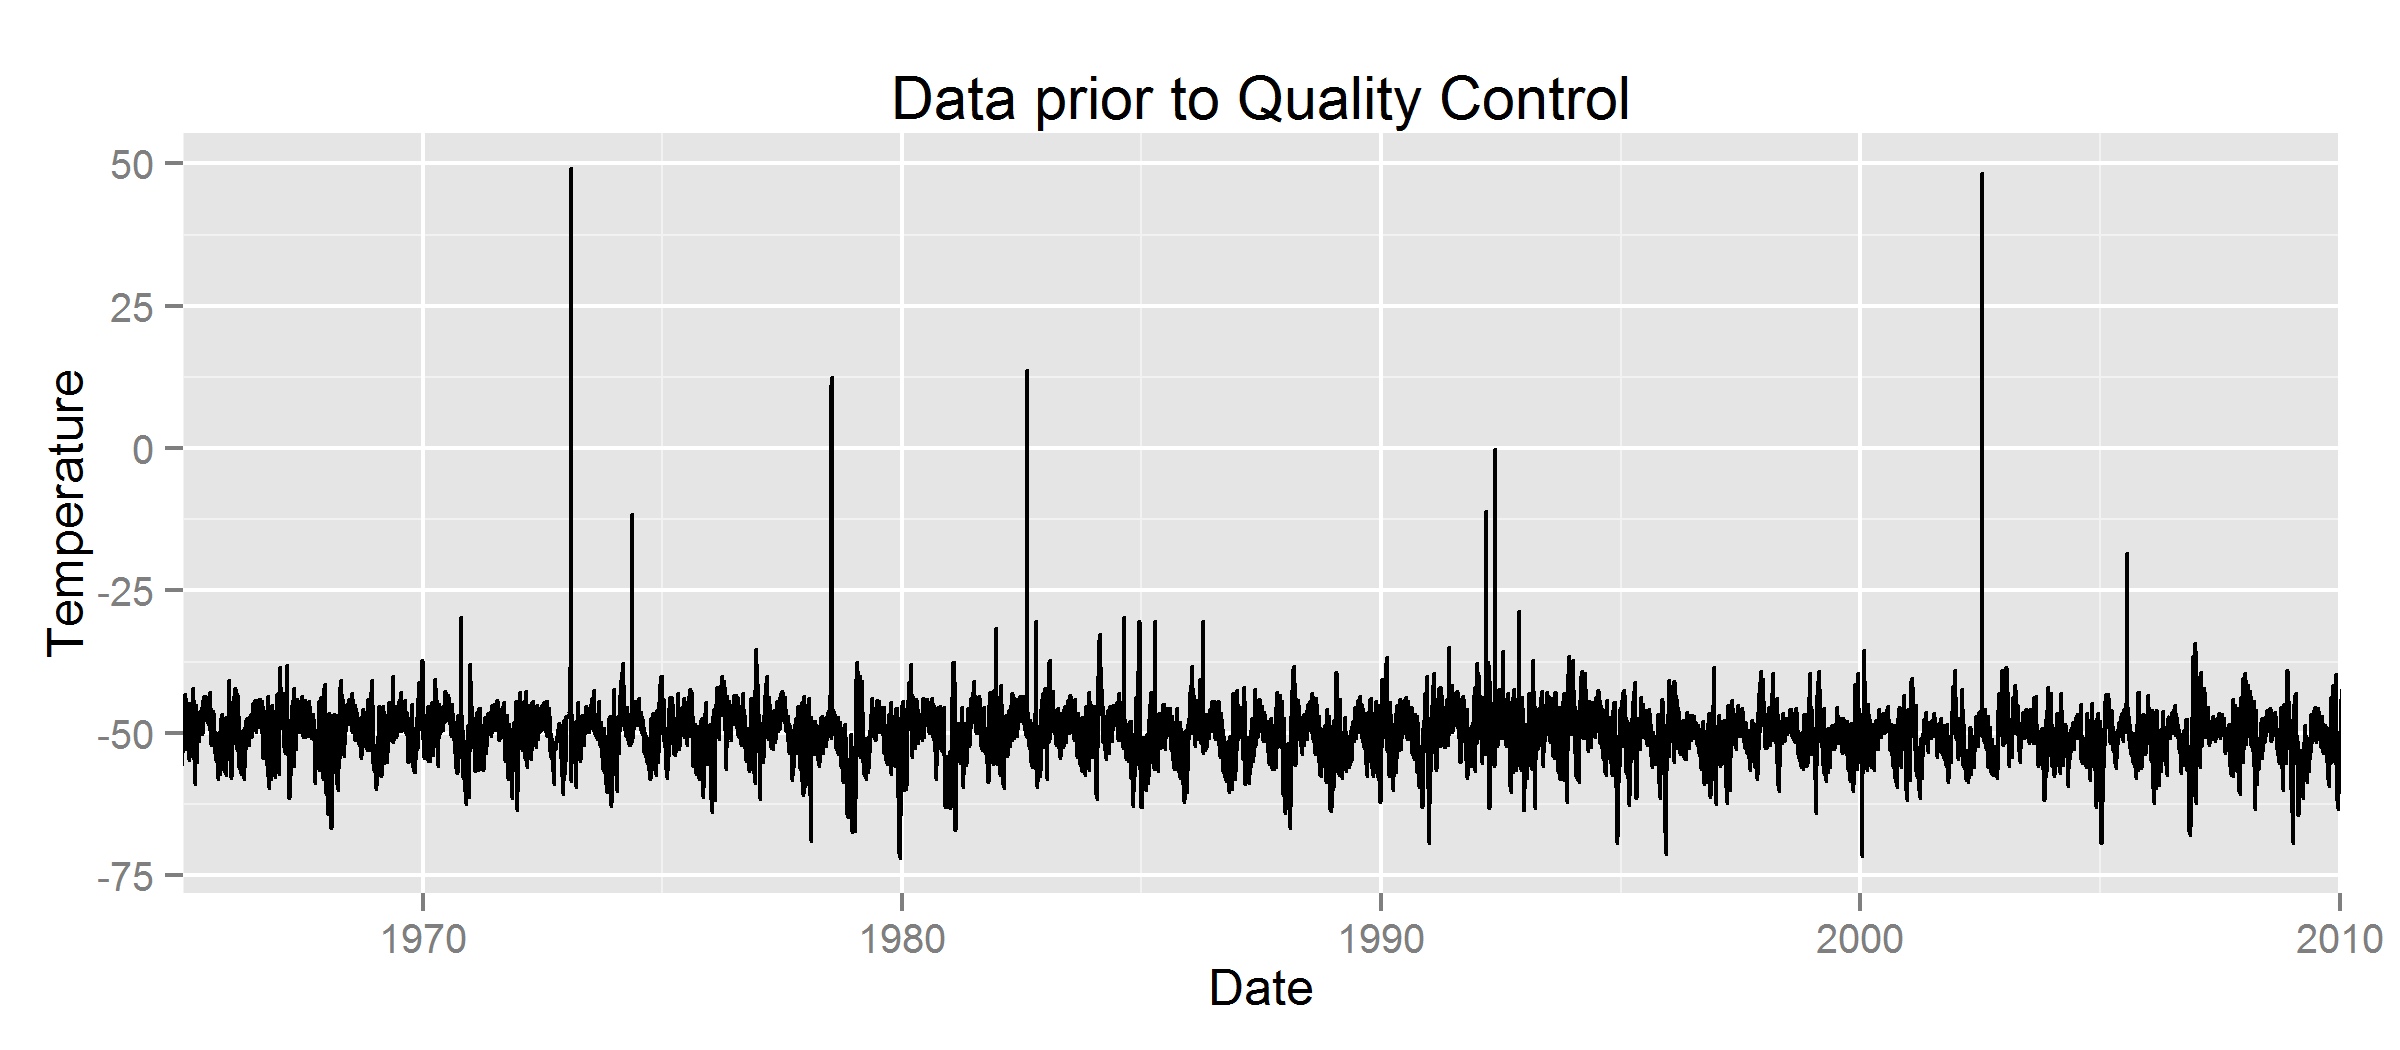
\includegraphics[width=.5\textwidth]{70219_Data_Unhomogenized_no_vlines} &
		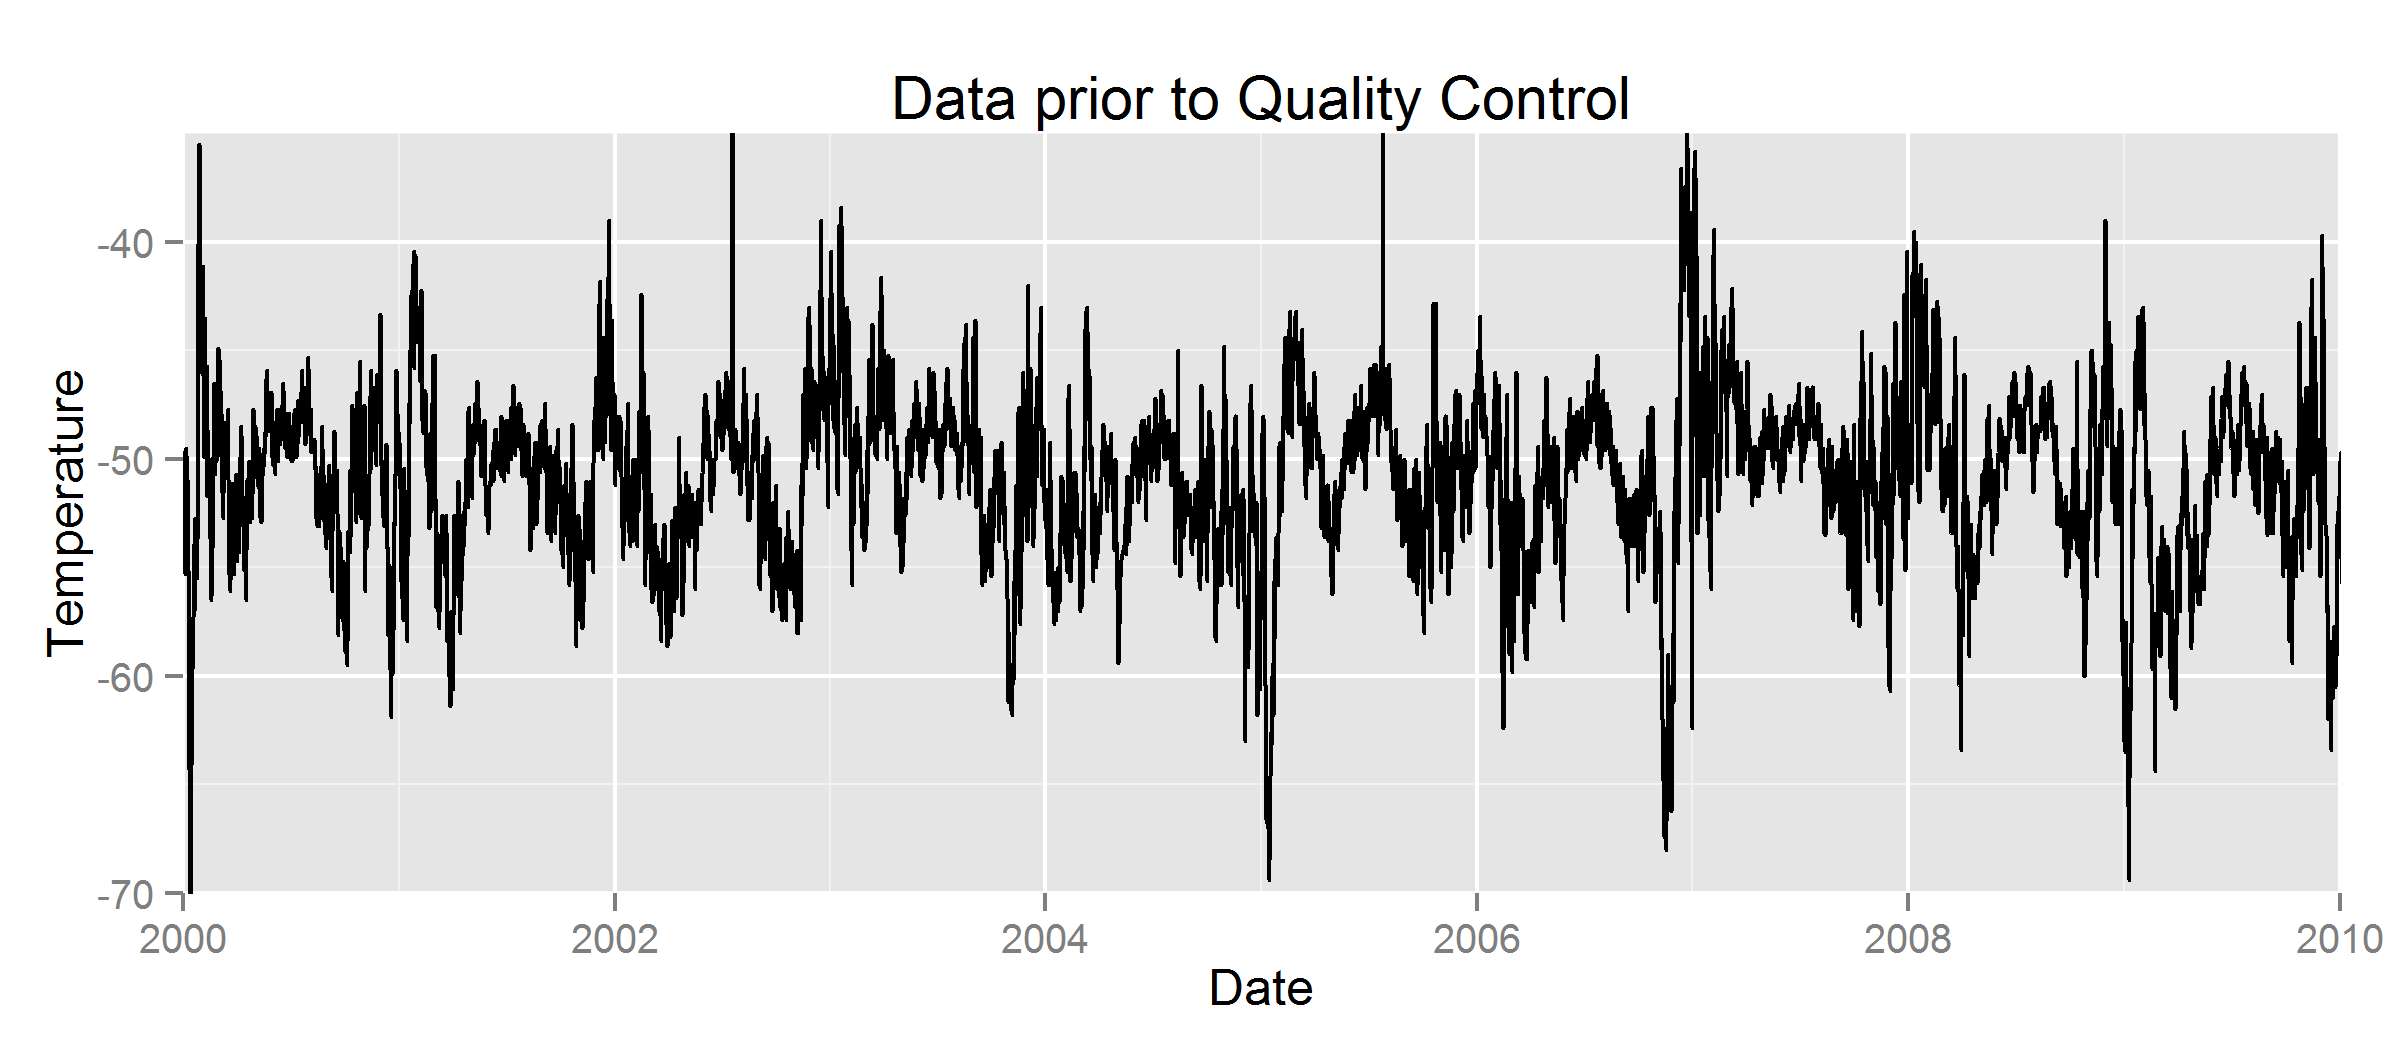
\includegraphics[width=.5\textwidth]{70219_Data_Unhomogenized_zoomed_no_vlines}
	\end{tabular}
	\caption{Temperature for Station 70219 plotted over time.  The right-hand image is the same as the first but zoomed in to the last ten years to show more detail.}
	\label{fig:BasicTS}
\end{figure}


\begin{figure}
	\centering
	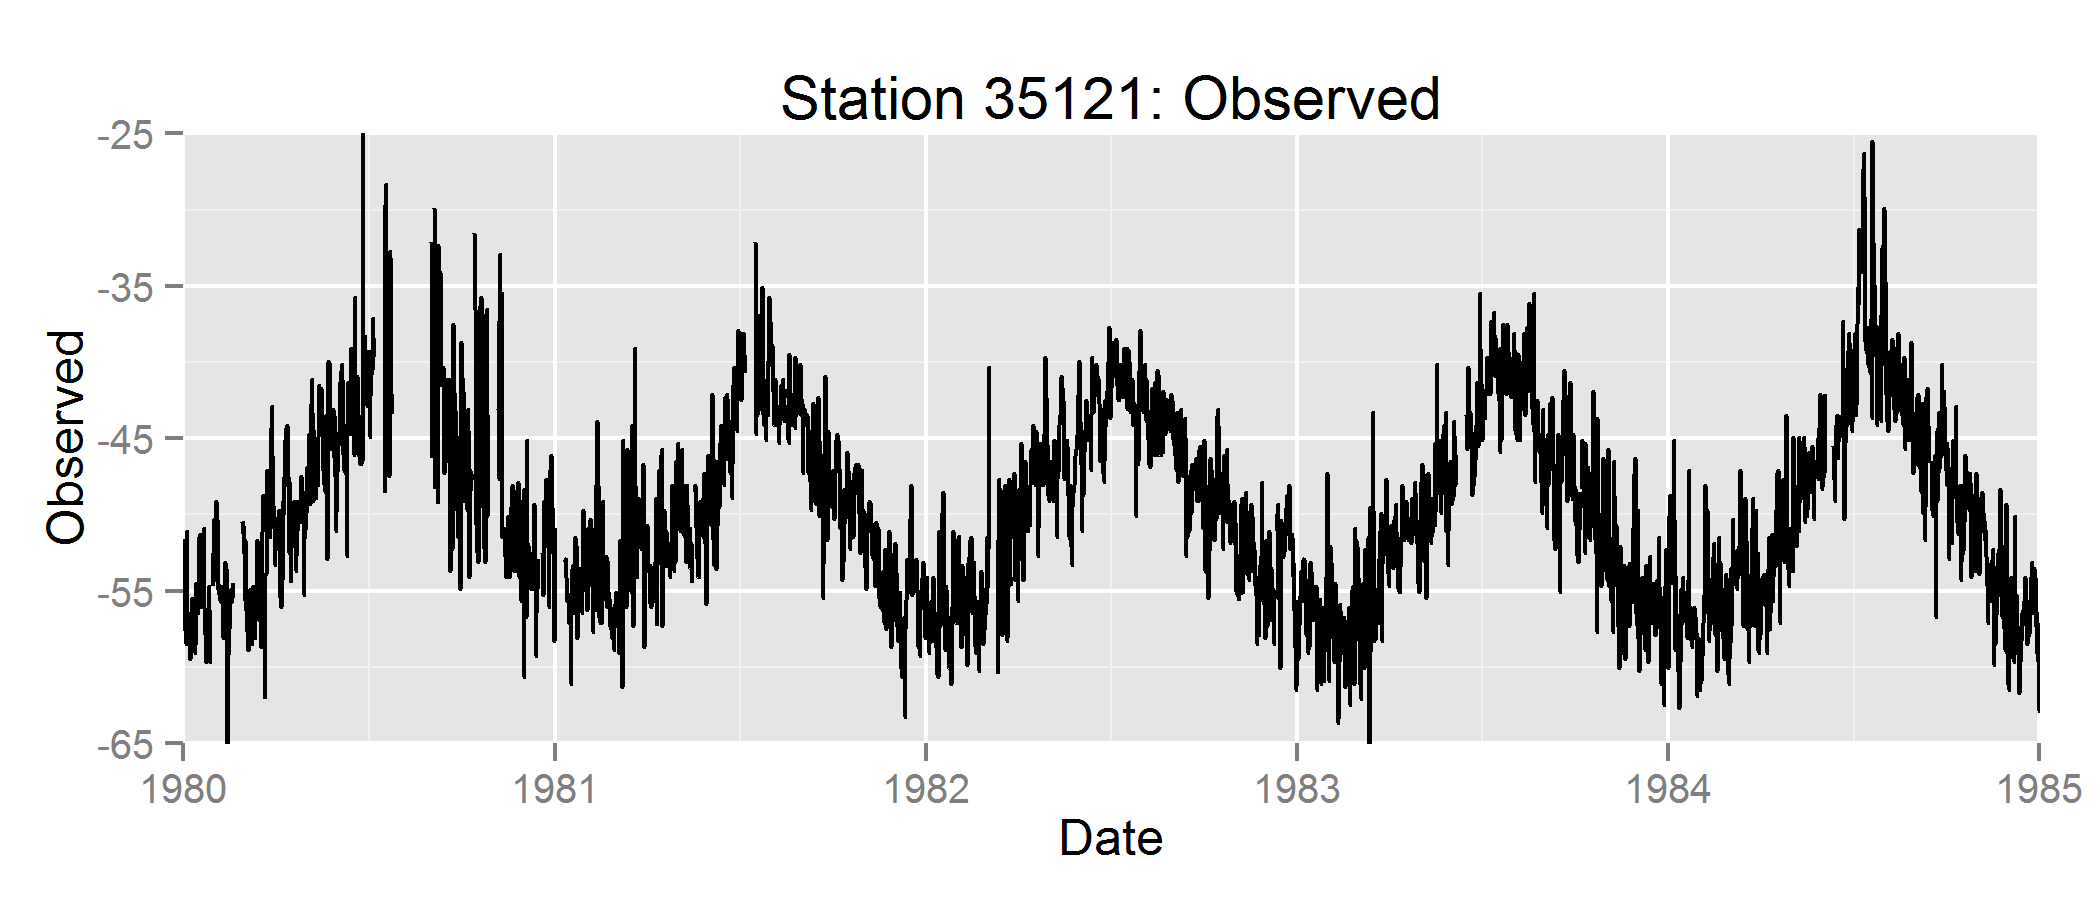
\includegraphics[width=.9\textwidth]{35121_time_series.png}\\
	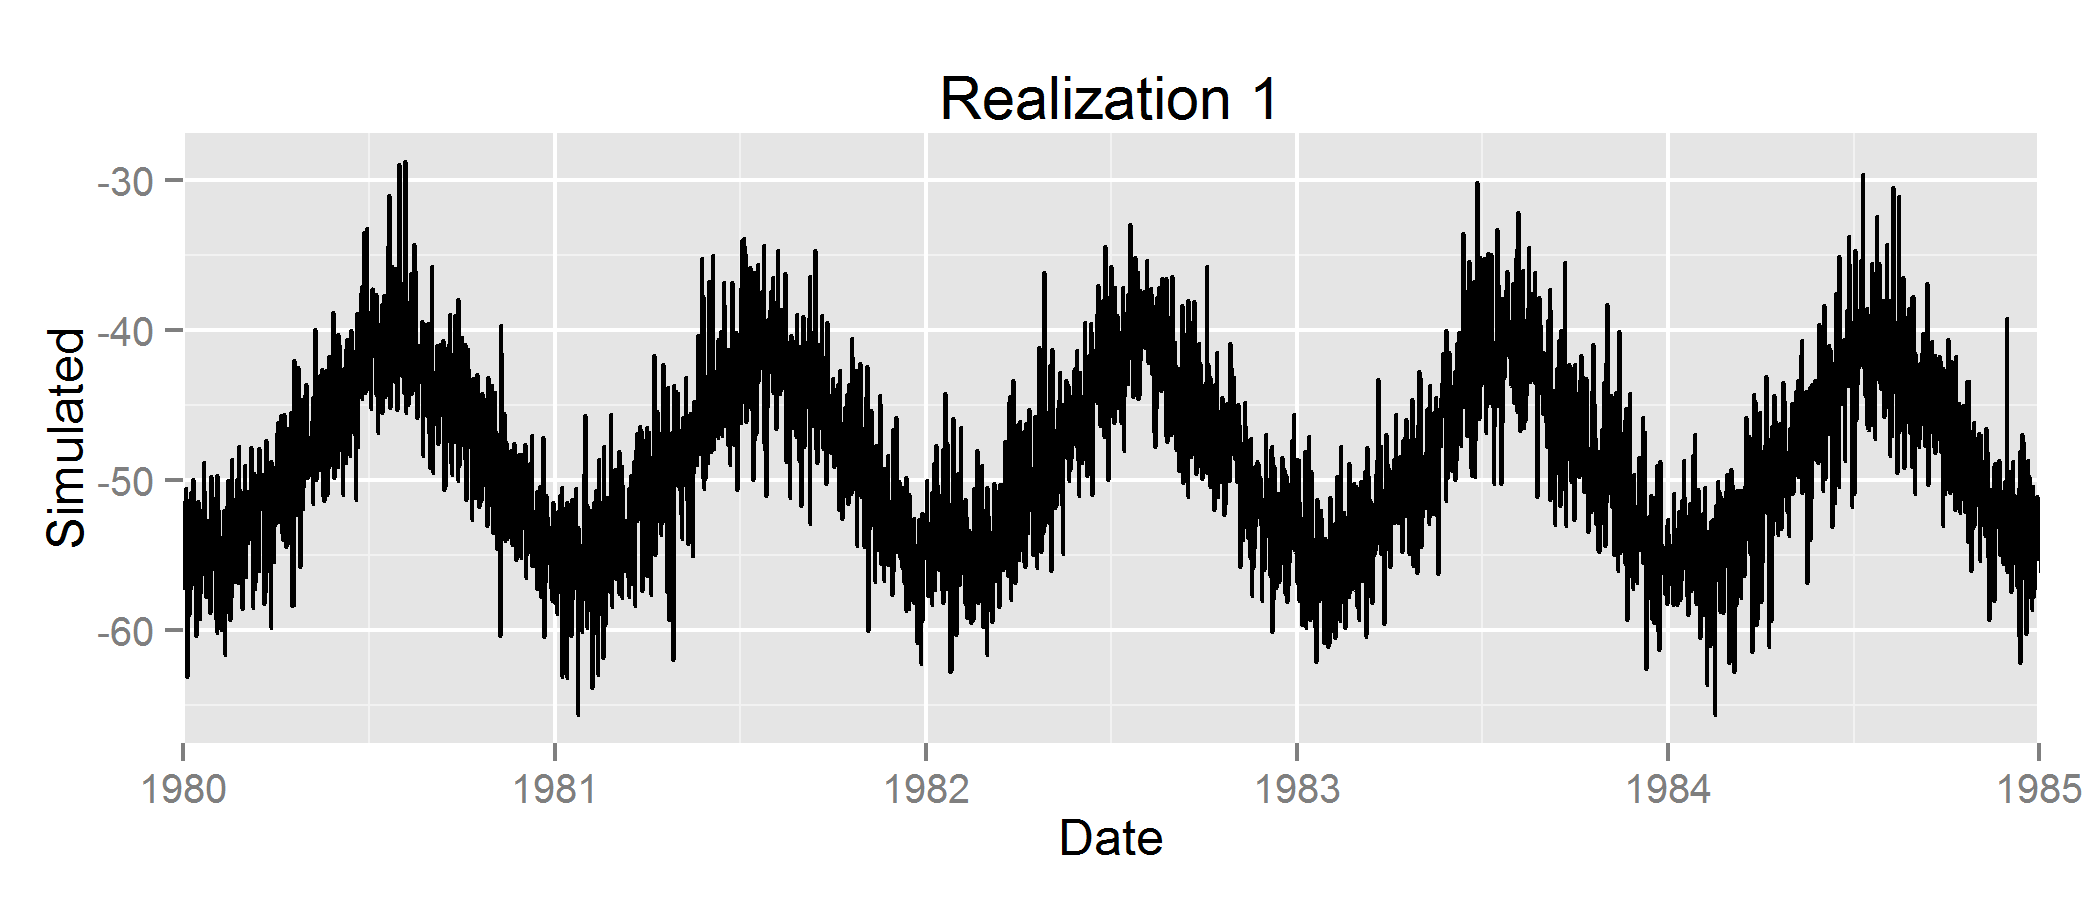
\includegraphics[width=.45\textwidth]{35121_simulated_1.png}
	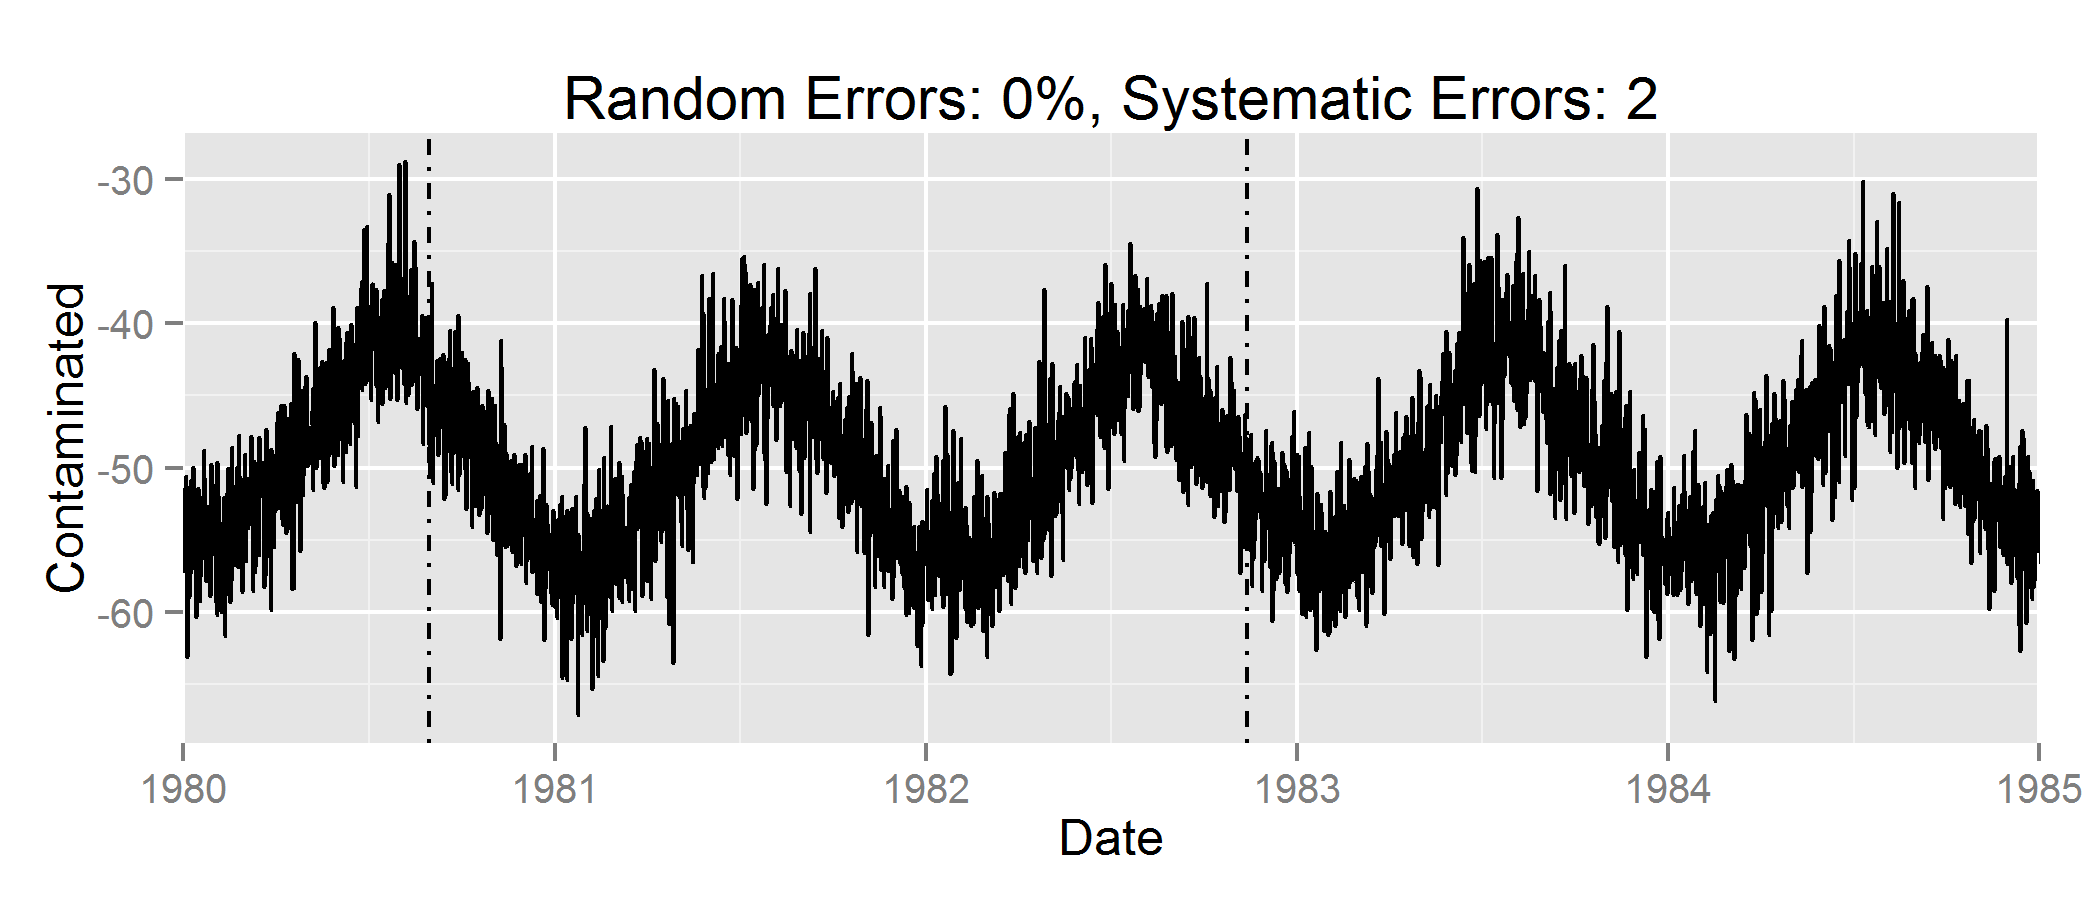
\includegraphics[width=.45\textwidth]{35121_contaminated_1.png}\\
	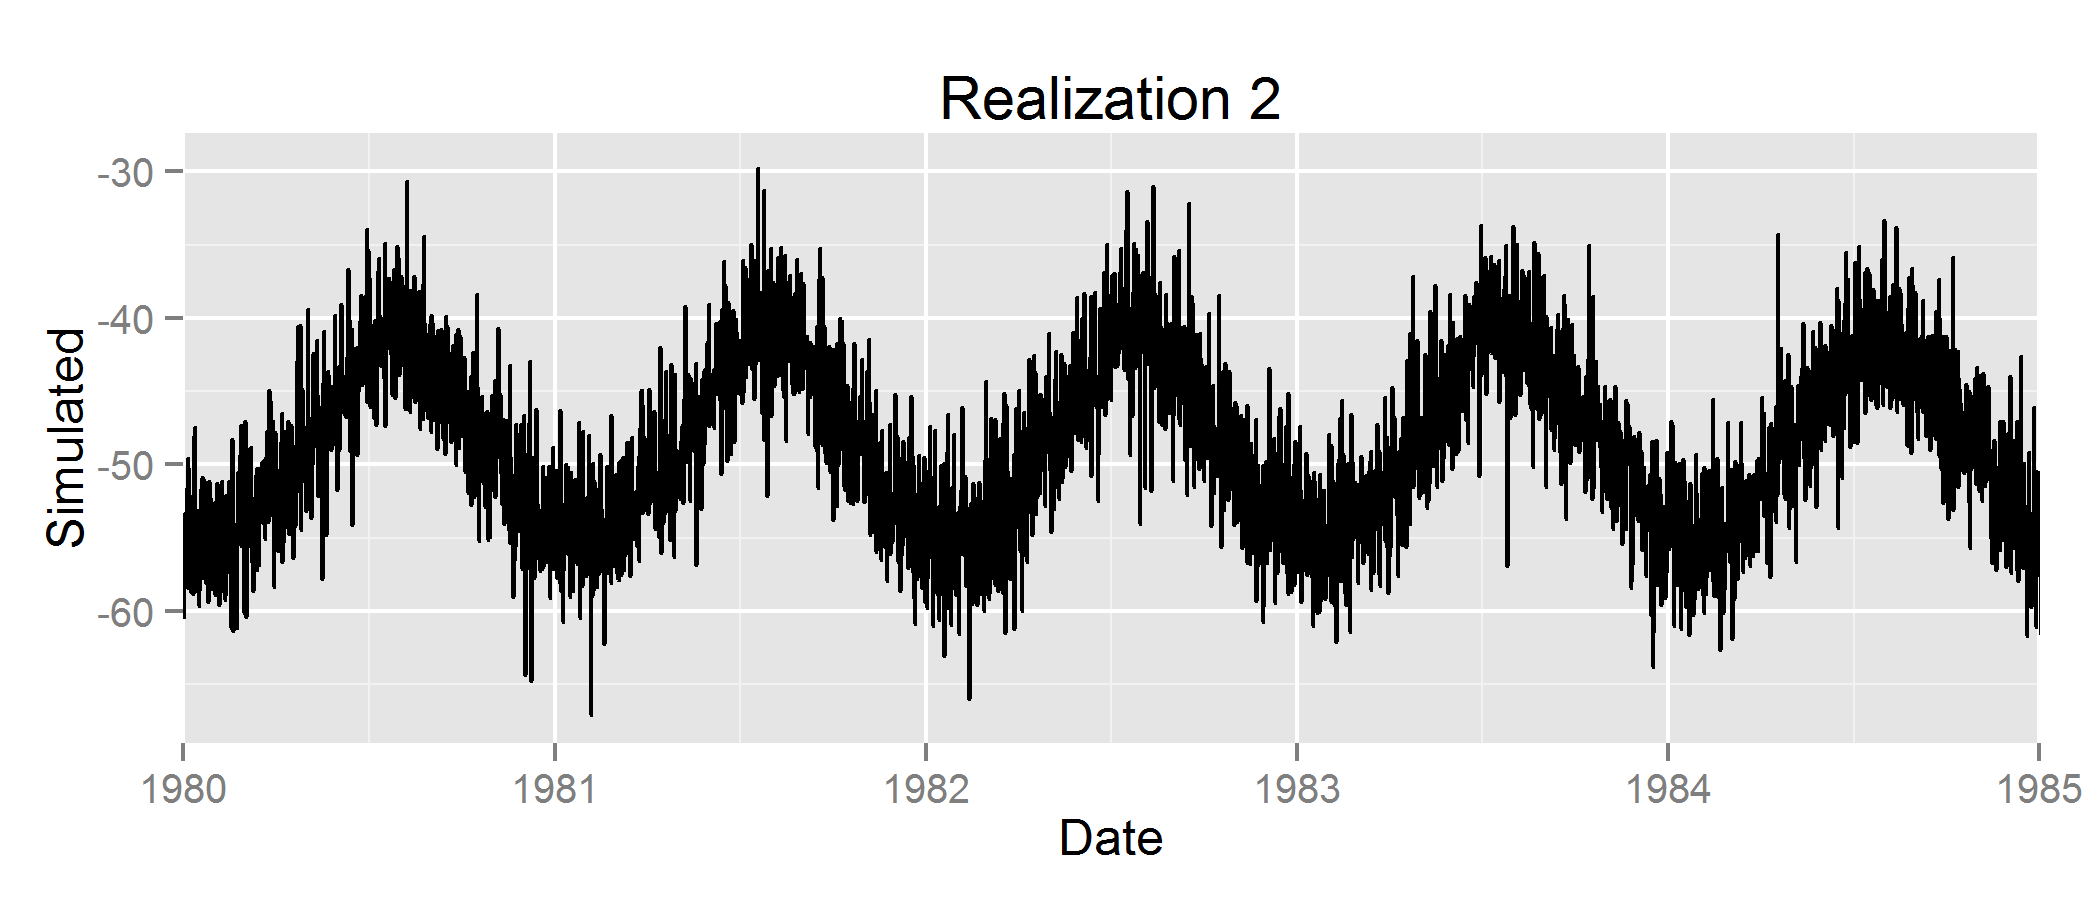
\includegraphics[width=.45\textwidth]{35121_simulated_2.png}
	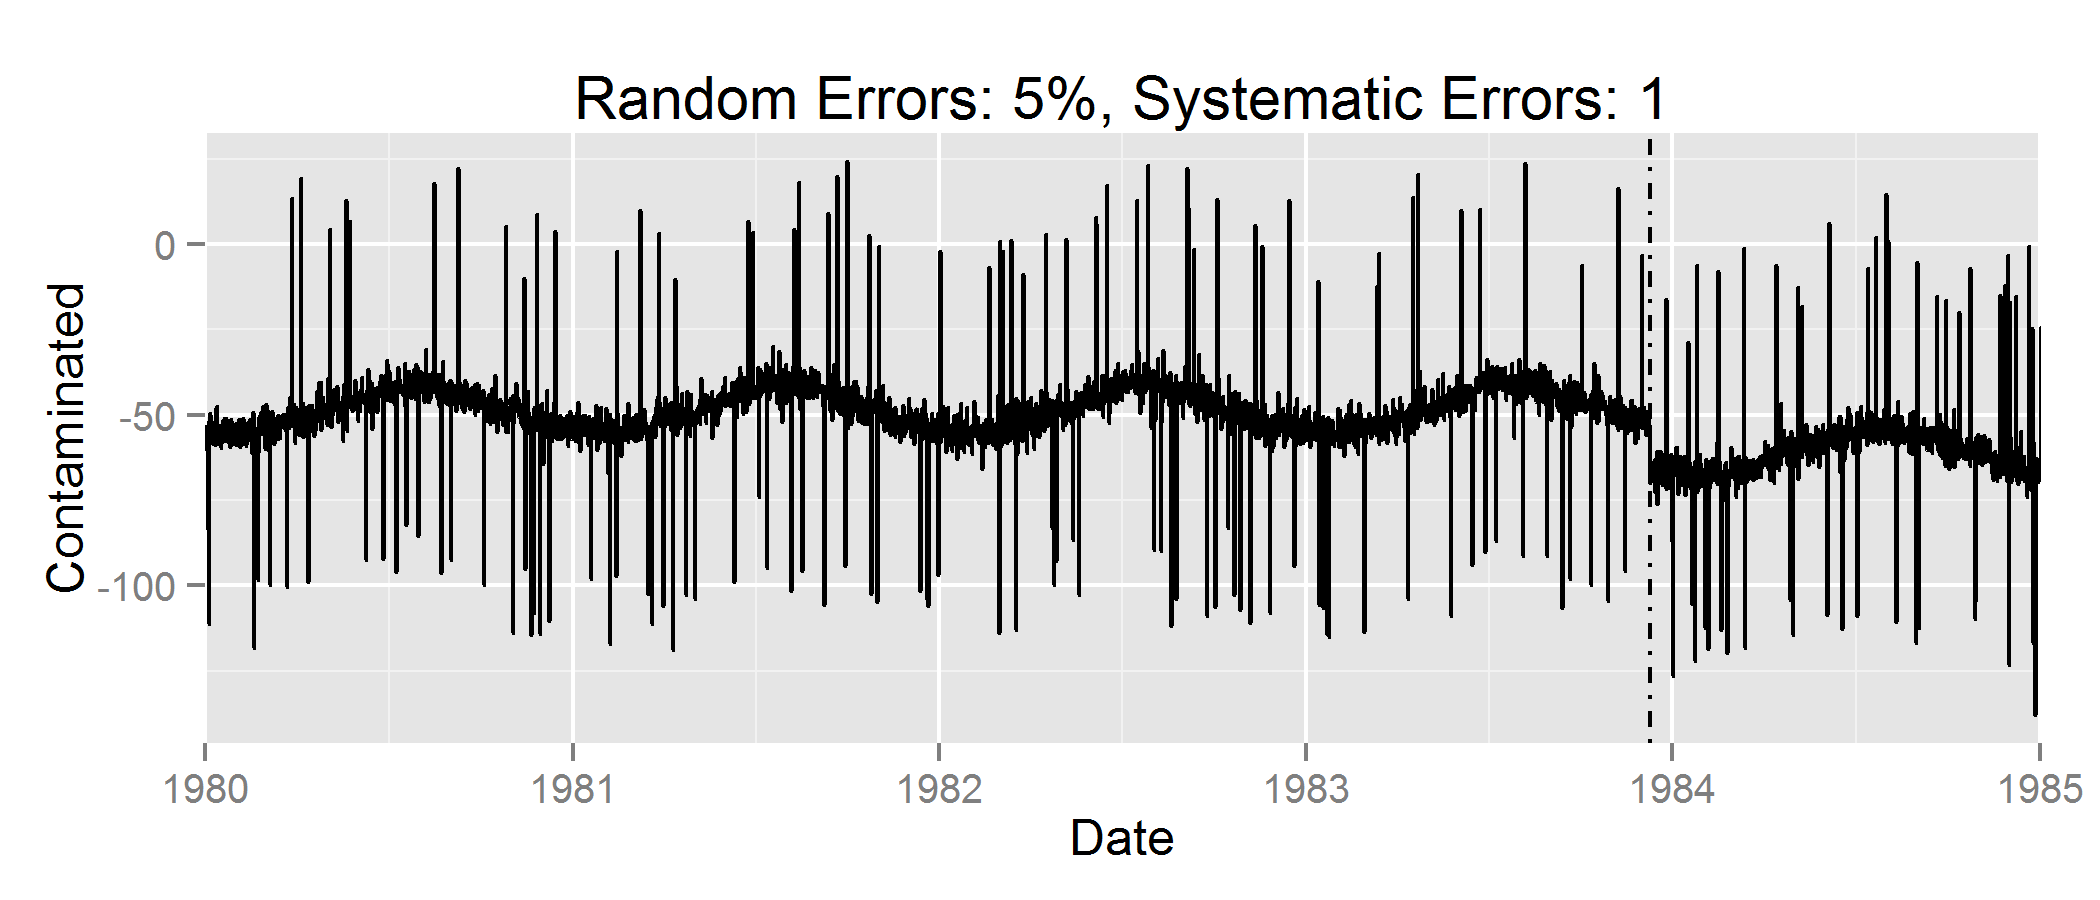
\includegraphics[width=.45\textwidth]{35121_contaminated_2.png}\\
	%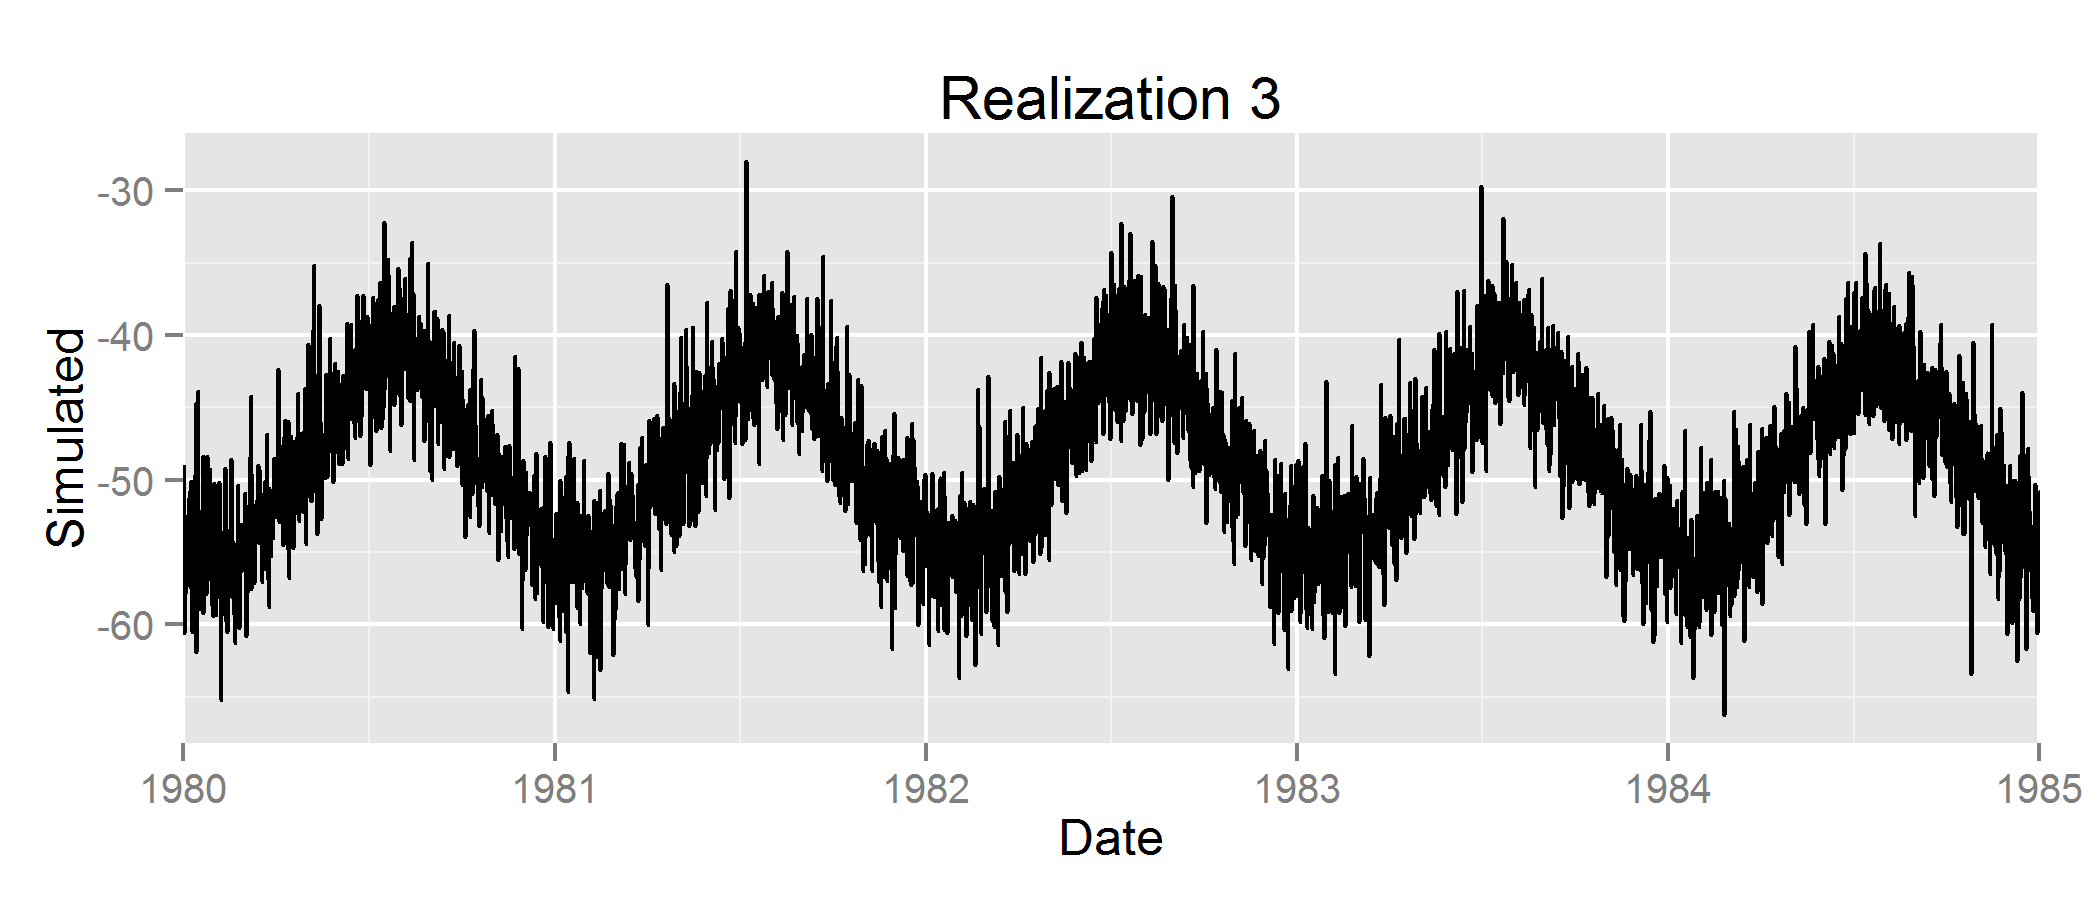
\includegraphics[width=.45\textwidth]{35121_simulated_3.png}
	%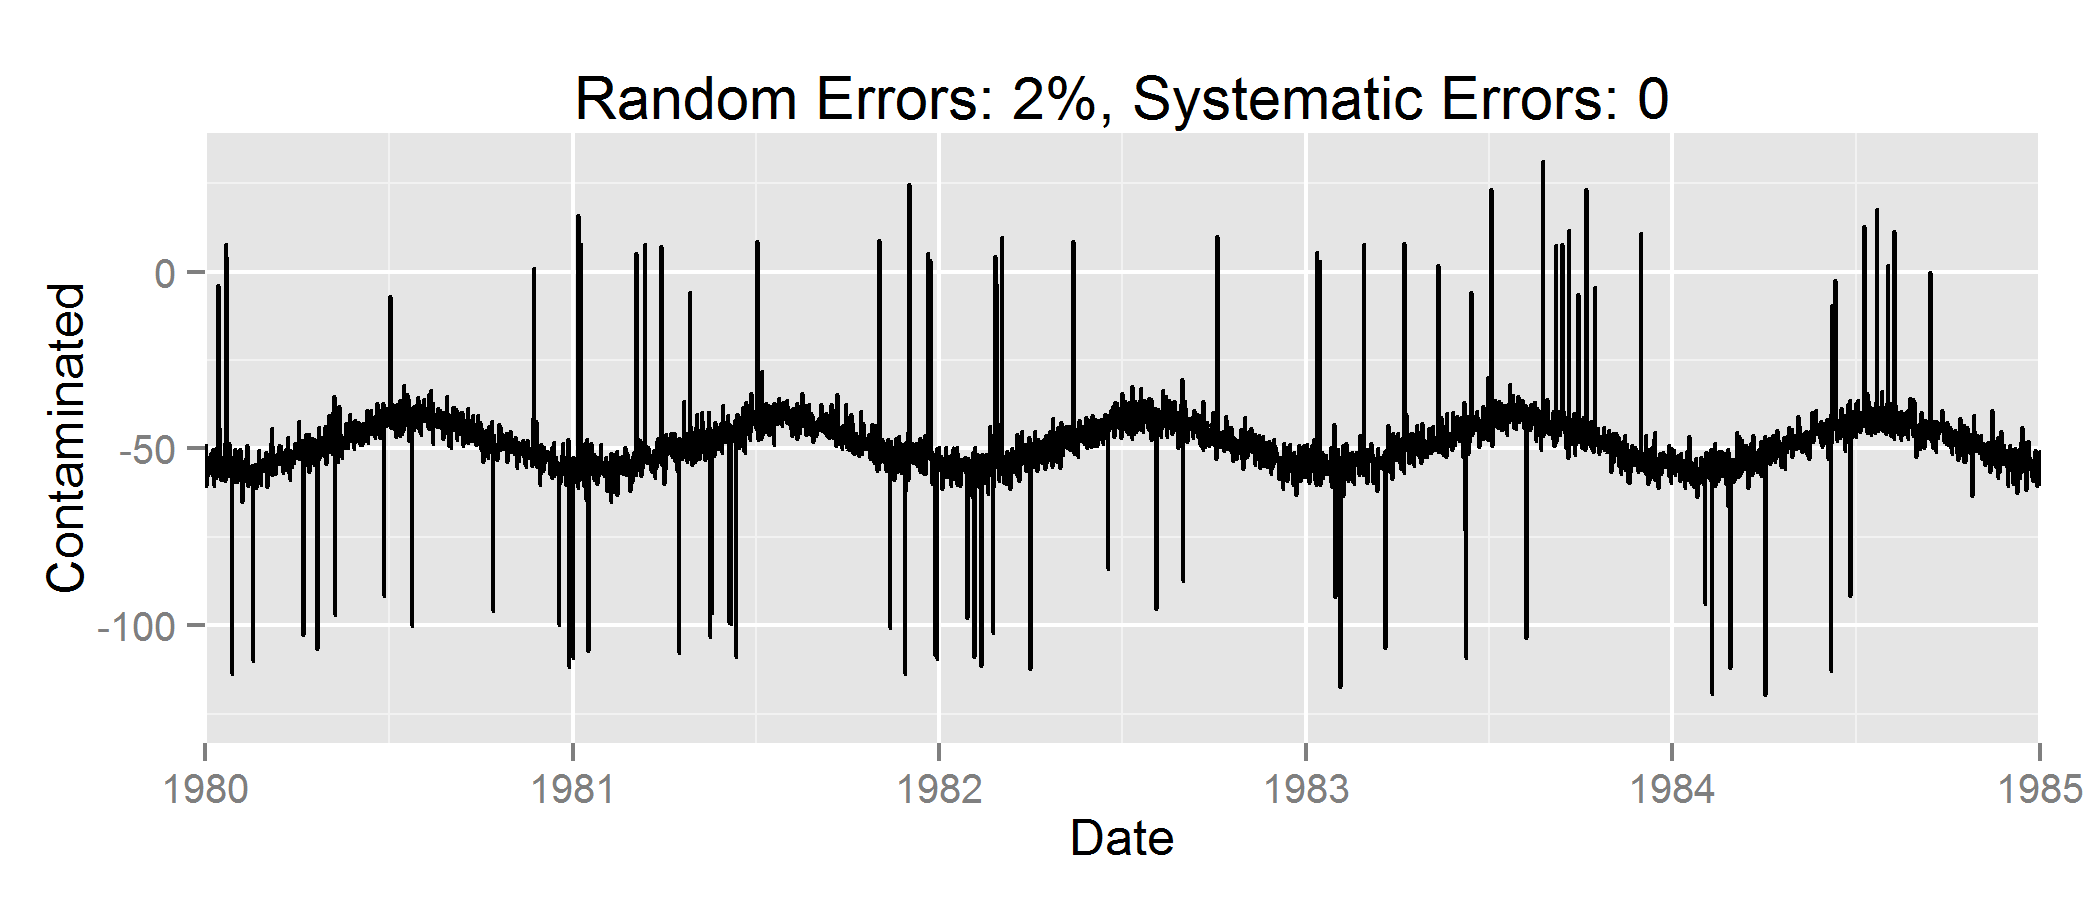
\includegraphics[width=.45\textwidth]{35121_contaminated_3.png}\\
	\caption{Time series plots of radiosonde temperature data from station 35121.  The top plot shows the observed time series, and the following two pairs show realizations of simulated datasets.  The plots on the left show the simulated data prior to contamination, and the right plots show the data after contamination with a combination of random and systematic errors.}
	\label{fig:simExample}
\end{figure}

\begin{figure}[h!]
	\centering
	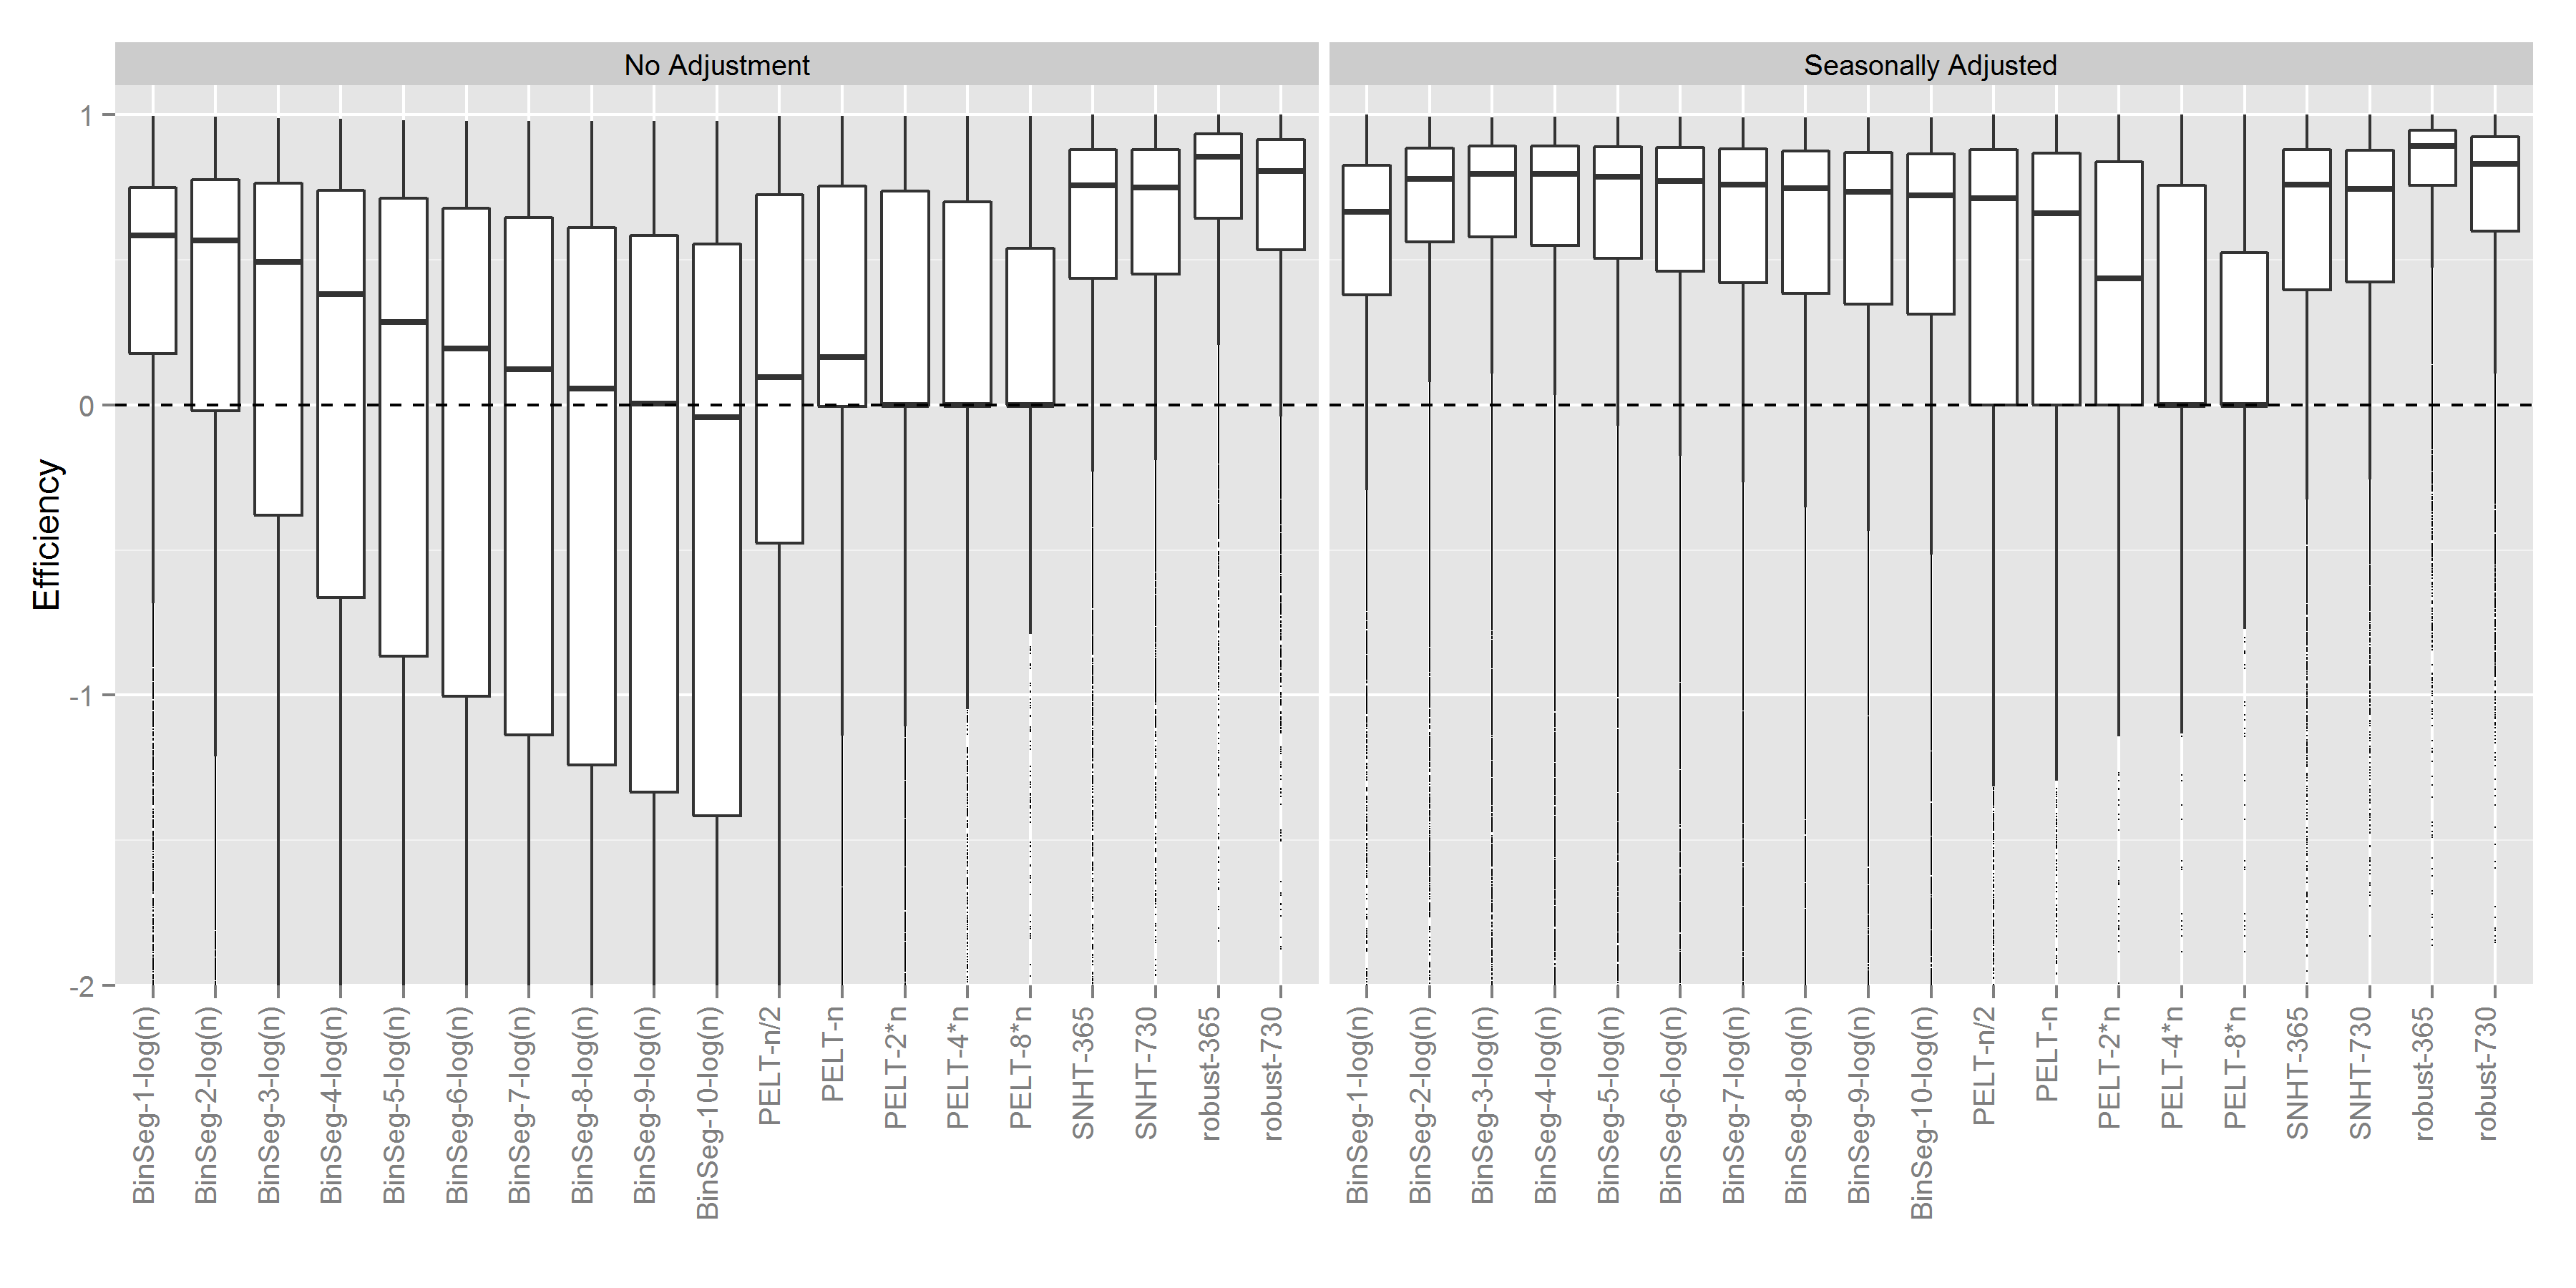
\includegraphics[width=\textwidth]{Efficiency_Model_Plot_BW_seas_adj.png}
	\caption{Boxplot of efficiency scores for the various homogenization algorithms.  Note that this graph is constrained to the efficiency range of $(-2,1)$ in order to show more detail.  The SNHT and the robust SNHT perform substantially  better than their alternatives.}
	\label{fig:homEfficiency}
\end{figure}

\begin{figure}[h!]
	\centering
	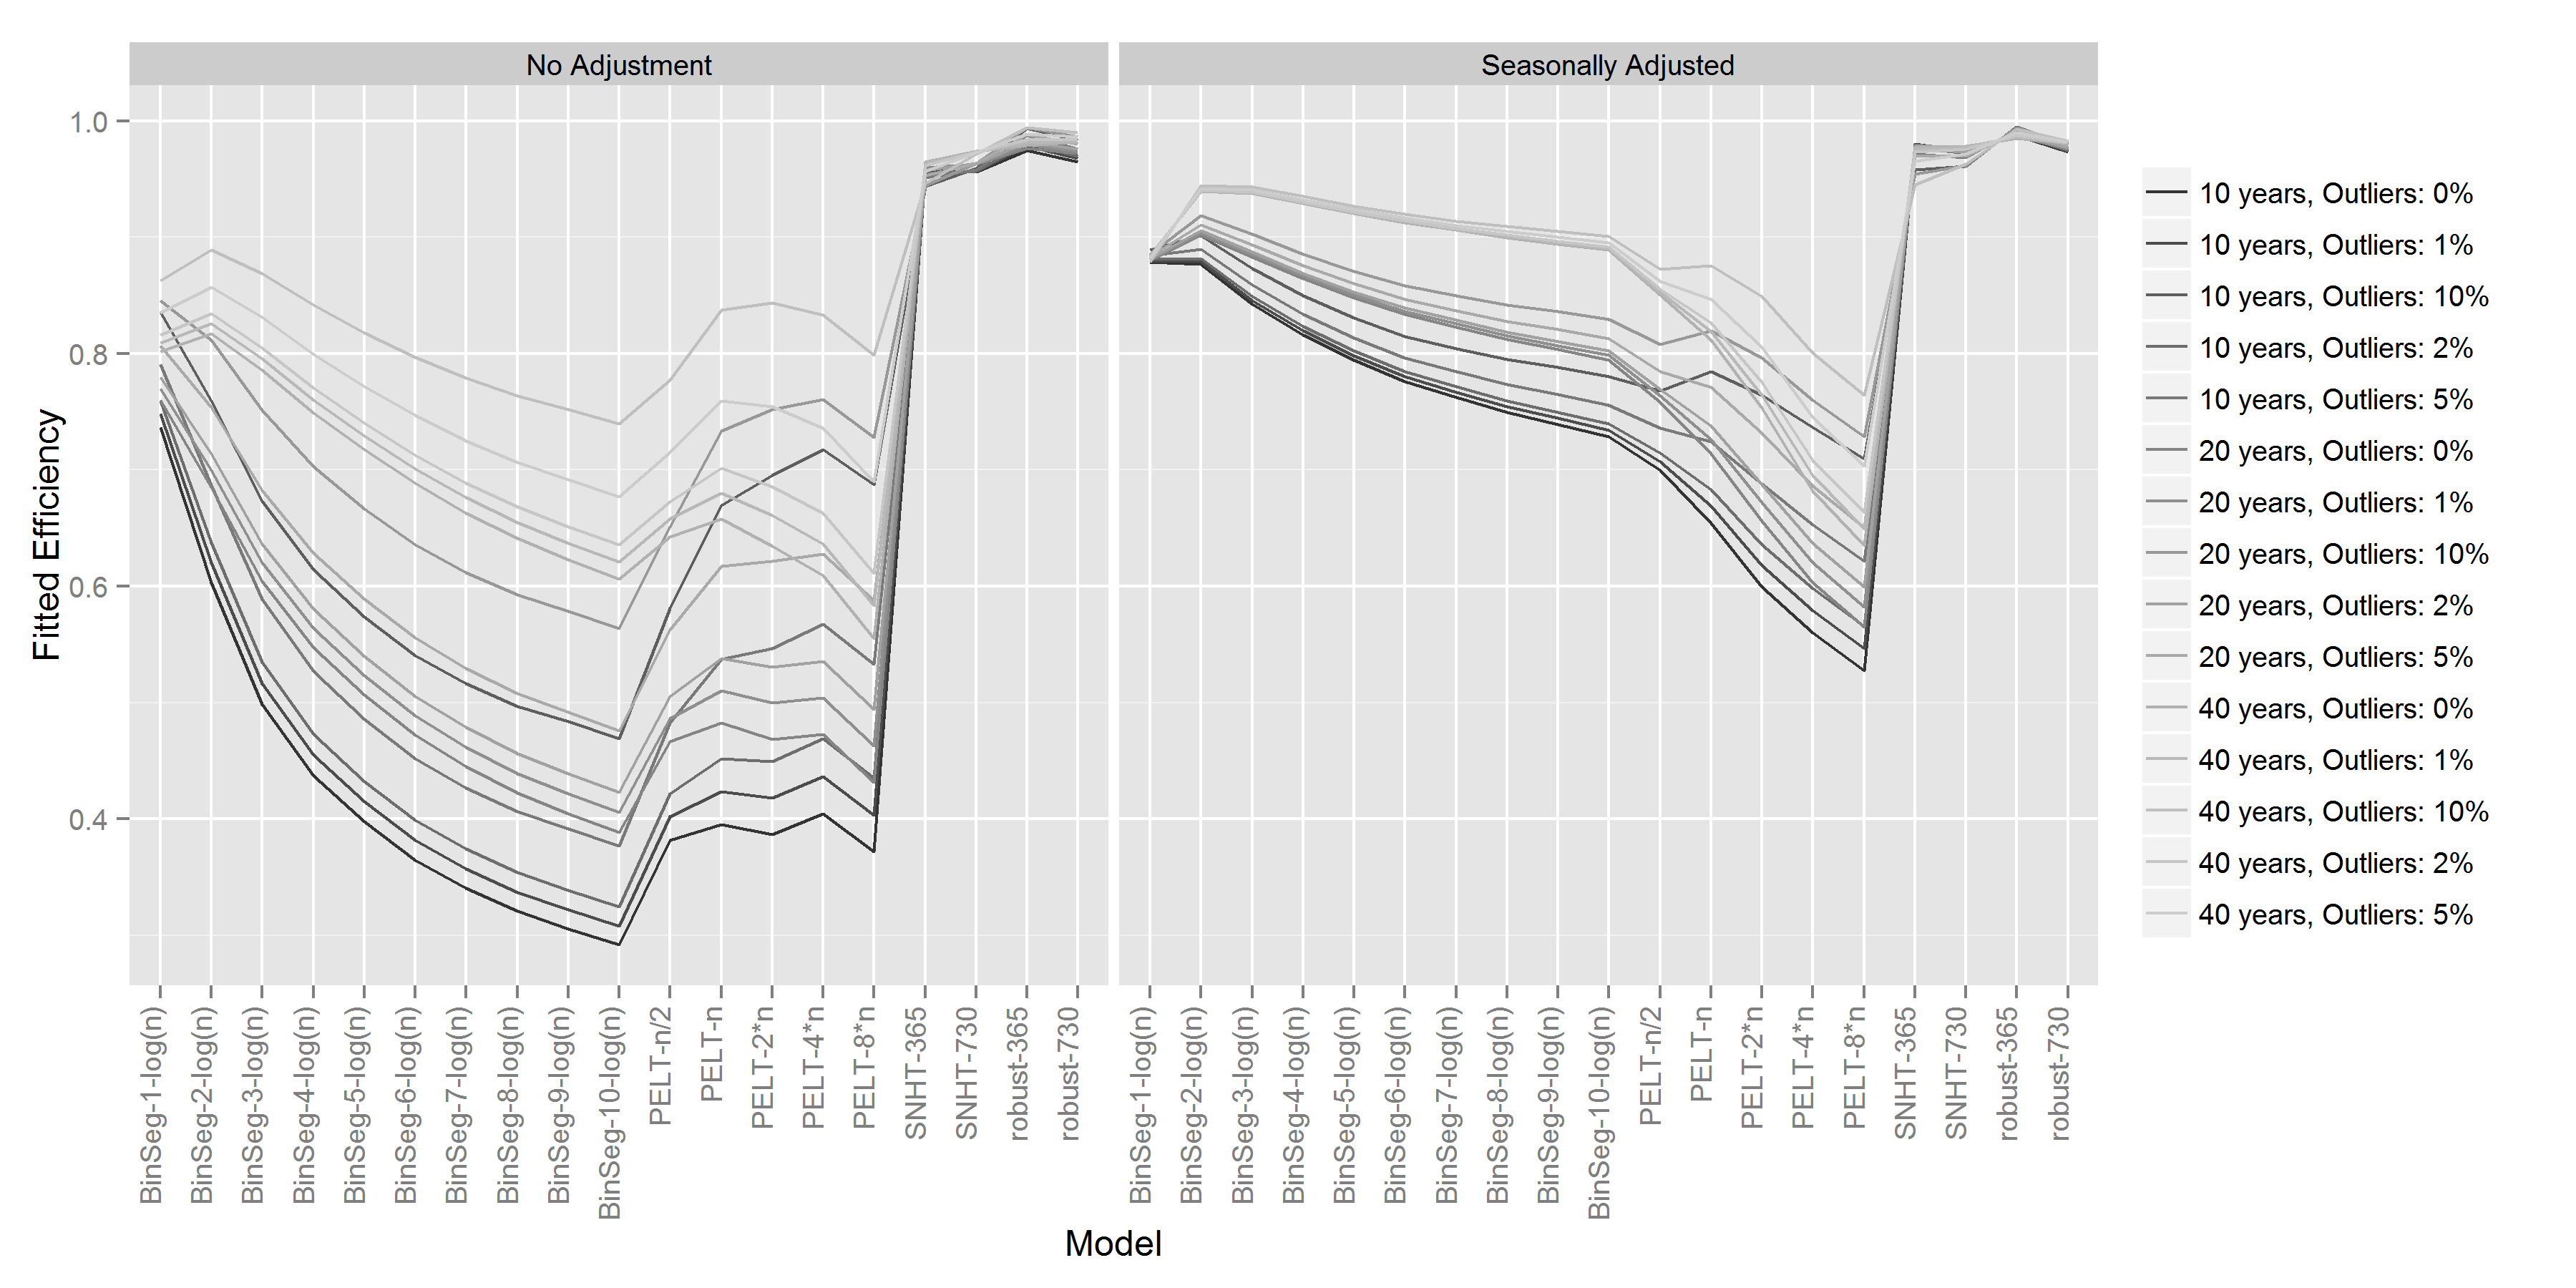
\includegraphics[width=\textwidth]{Efficiency_Model_Plot_BW_seasonal.png}
	\caption{This graph depicts the estimated probability that the efficiency exceeds one from the efficiency logistic regression model.  Each line represents a different simulation configuration (number of years simulated and outlier contamination rates).  There is substantial variability among the different simulations, but  the SNHT and robust SNHT models perform better than the alternatives in all simulated configurations, and the efficiency improves with sample size.}
	\label{fig:homFitEff}
\end{figure}

\begin{figure}[h!]
	\centering
	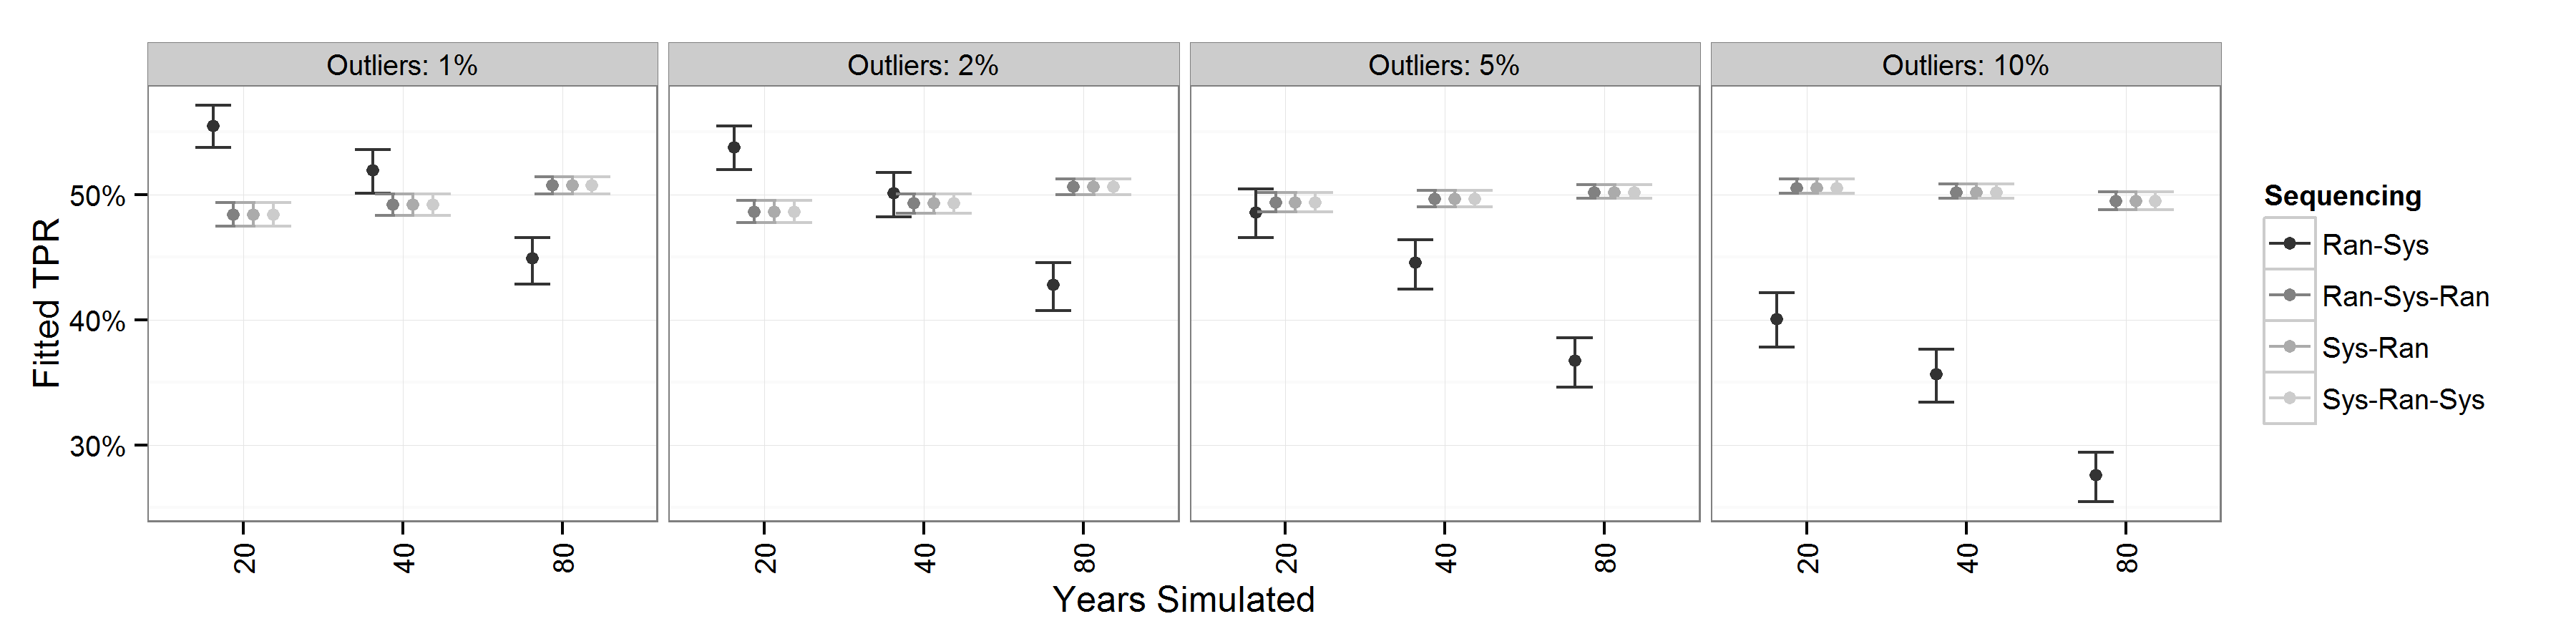
\includegraphics[width=\textwidth]{TPR_Order_Plot_BW}
	\caption{This graph depicts the estimated TPR from the logistic regression model.  The dot in each error bar is the estimated TPR averaged over all station and pressure level combinations.  The maximum (minimum) of the error bar is the highest (lowest) TPR obtained across all station and pressure level combinations.}
	\label{fig:fitTPR}
\end{figure}

\begin{figure}[h!]
	\centering
	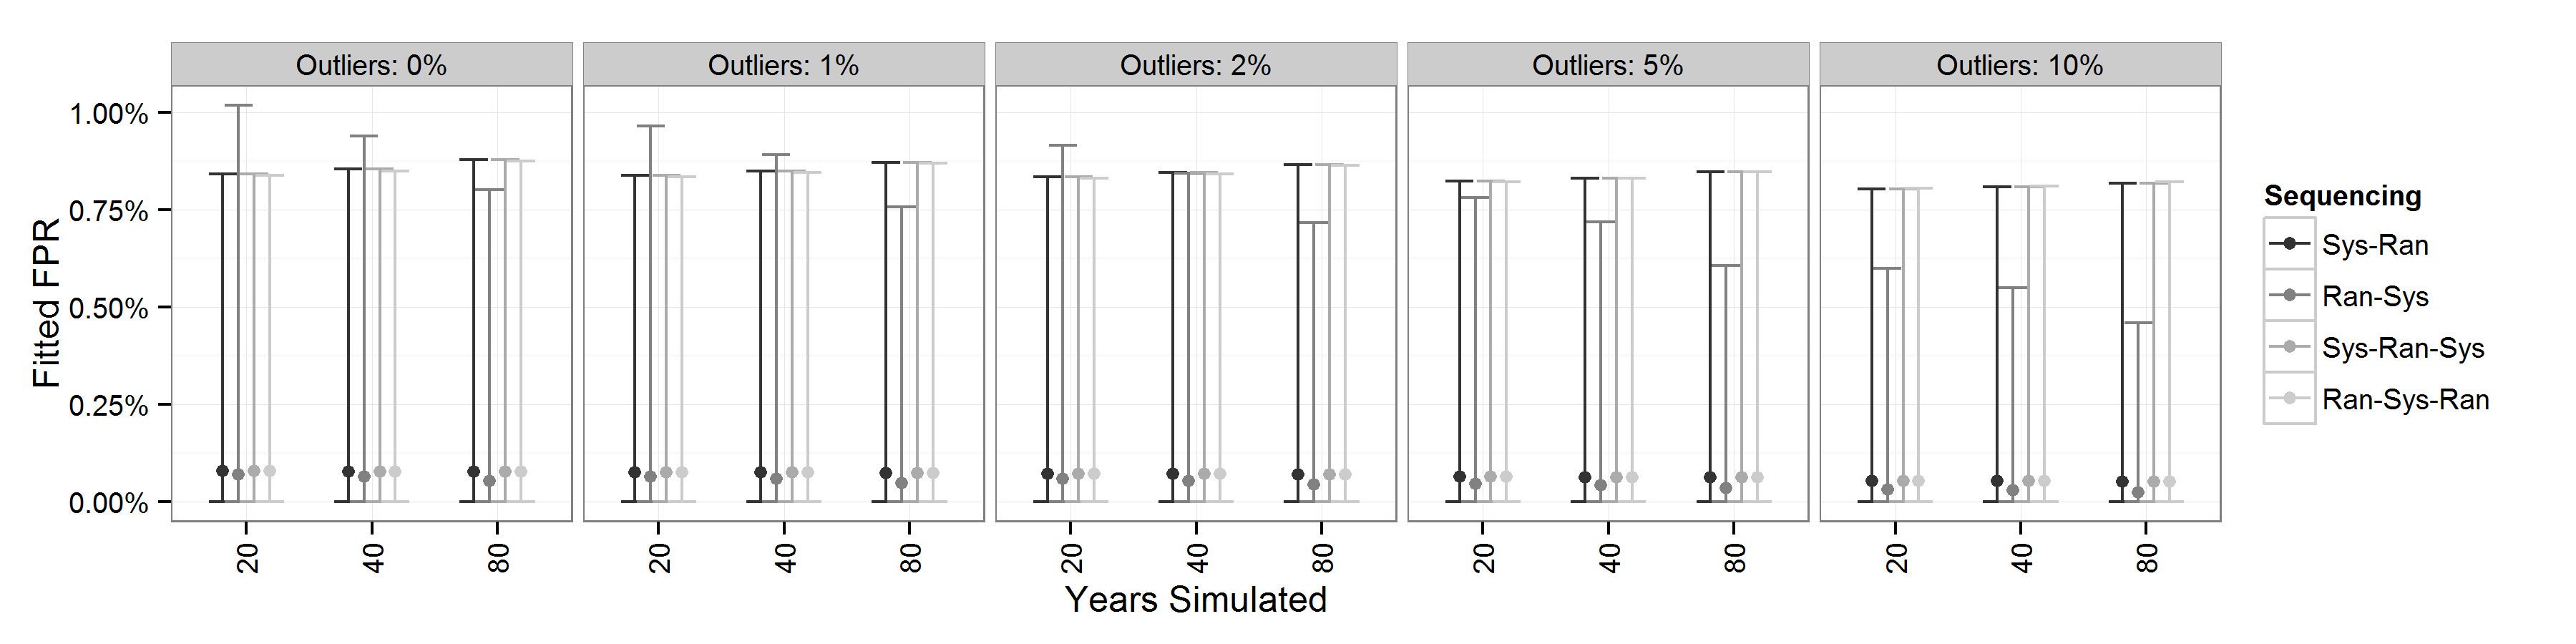
\includegraphics[width=\textwidth]{FPR_Order_Plot_BW}
	\caption{This graph depicts the estimated FPR from the logistic regression model.  The dot in each error bar is the estimated FPR averaged over all station and pressure level combinations.  The maximum (minimum) of the error bar is the highest (lowest) FPR obtained across all station and pressure level combinations.  }
	\label{fig:fitFPR}
\end{figure}


\begin{figure}[h!]
	\centering
	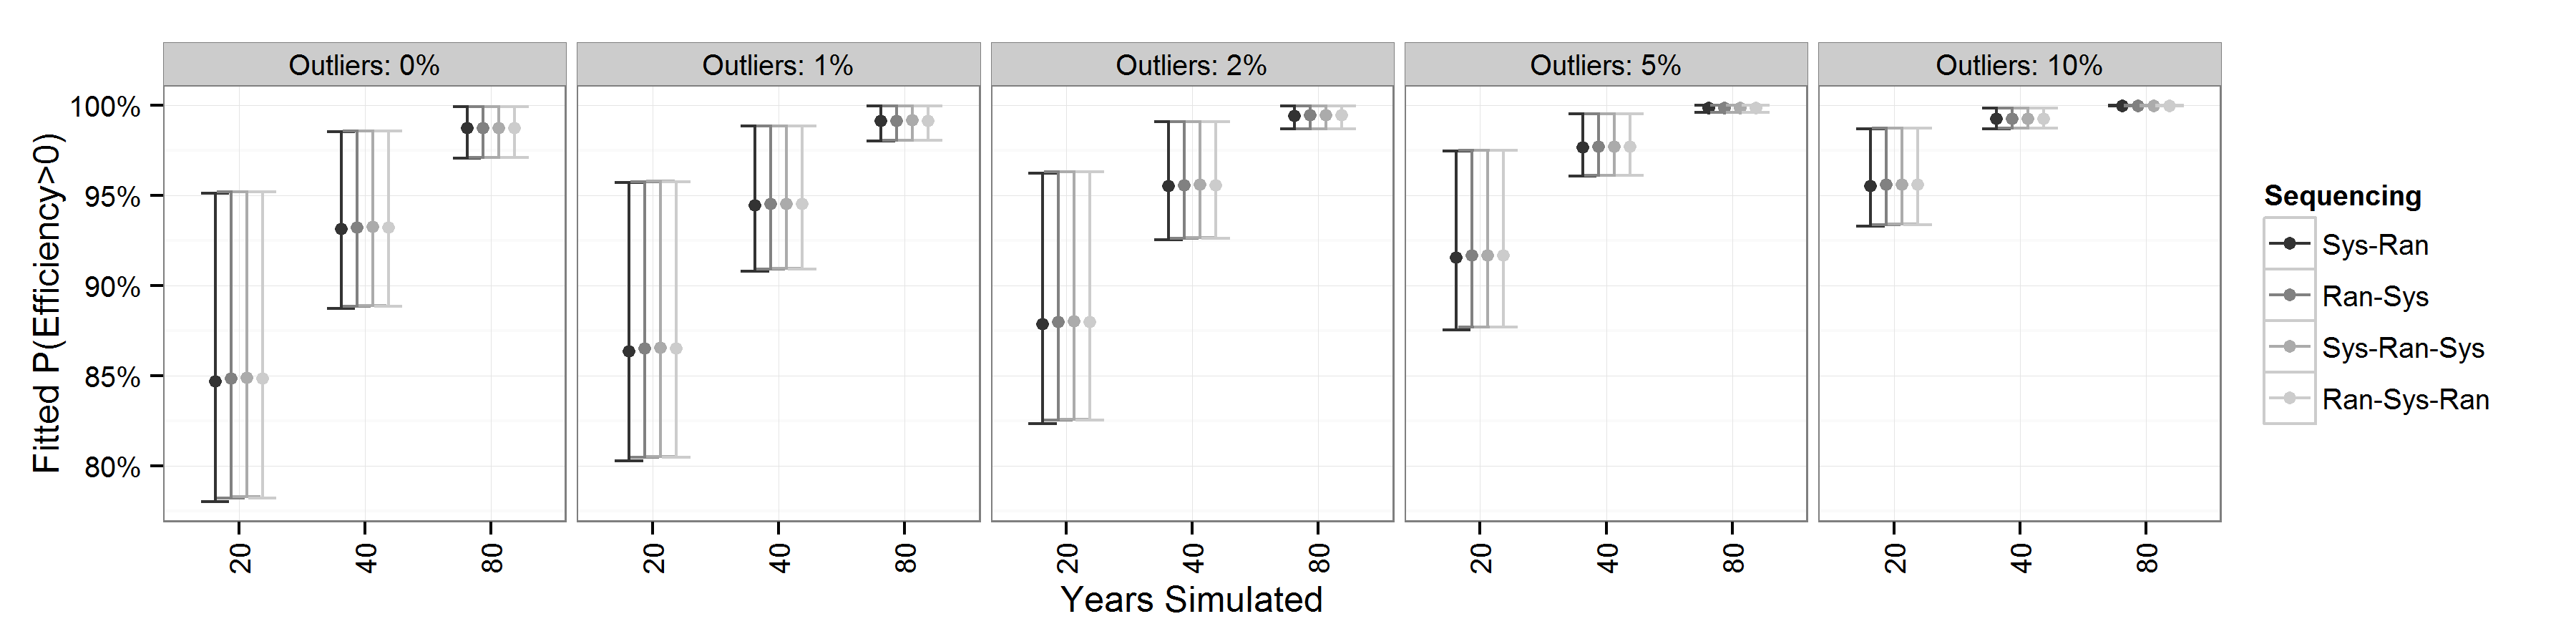
\includegraphics[width=\textwidth]{Efficiency_Order_Plot_BW}
	\caption{This graph depicts the estimated efficiency from the logistic regression model.  The middle of each error bar is the estimated efficiency averaged over all station and pressure level combinations.  The maximum (minimum) of the error bar is the highest (lowest) efficiency obtained across all station and pressure level combinations.}
	\label{fig:fitEffOrd}
\end{figure}


\begin{figure}
	\centering
	\includegraphics[width=.9\textwidth]{"70219_Data_Unhomogenized_zoomed"}
	\includegraphics[width=.9\textwidth]{"70219_Data_Homogenized_zoomed"}
	\includegraphics[width=.9\textwidth]{"70219_Data_Homogenized"}	
	\caption{Time series plot of the radiosonde temperature data at station 70219 (Bethel, Alaska, USA).  The top plot shows the data prior to the quality control algorithm, and the other two show the data after for a subset (middle) and the entire record (bottom).  Dashed vertical lines indicate detected change points, numbers in the top panel indicate the magnitude of the corresponding change point, and dots indicate detected random errors.}
	\label{fig:caseStudy}
\end{figure}

%%%%%%%%%%%%%%%%%%%%
\end{document}
%%%%%%%%%%%%%%%%%%%%
